\subsection*{Общая характеристика работы}

\newcommand{\actuality}{\underline{\textbf{Актуальность темы.}}}
\newcommand{\aim}{\underline{\textbf{Целью}}}
\newcommand{\tasks}{\underline{\textbf{задачи}}}
\newcommand{\defpositions}{\underline{\textbf{Основные положения, выносимые на~защиту:}}}
\newcommand{\novelty}{\underline{\textbf{Научная новизна:}}}
\newcommand{\influence}{\underline{\textbf{Практическая значимость}}}
\newcommand{\reliability}{\underline{\textbf{Достоверность}}}
\newcommand{\probation}{\underline{\textbf{Апробация работы.}}}
\newcommand{\contribution}{\underline{\textbf{Личный вклад.}}}
\newcommand{\publications}{\underline{\textbf{Публикации.}}}

{\actuality} Процесс упругого когерентного рассеяния нейтрино (УКРН) на атомных ядрах предсказан Стандартной Моделью (СМ) в 1974 году как в работах зарубежных ученых~\cite{Freedman}, так и отечественных~\cite{Kopeliovich:1974mv}, однако только в 2017 году был зарегистрирован экспериментально~\cite{COHERENT:2017ipa}. Такой большой временной промежуток связан, прежде всего, с очень малым энерговыделением (единицы-десятки кэВ на ядро) в рабочей среде детектора.
\par Процесс УКРН имеет фундаментальное значение для описания процессов формирования Вселенной и эволюции звёзд. Отклонения измеренного сечения взаимодействия УКРН от предсказаний СМ могут быть использованы для поиска явлений за ее пределами. Кроме того, процесс УРКН можно использовать для изучения ядерных форм-факторов и магнитного момента нейтрино. Также разработка технологий регистрации УКРН может позволить добиться существенного прогресса в области удаленного мониторинга ядерных реакторов, что имеет важное практическое значение. На данный момент технология нейтринного мониторинга ядерных реакторов основана на эффекте обратного бета-распада~\cite{Rusov}, однако сечение процесса УКРН в несколько сотен раз больше. Это свойство потенциально может позволить мониторировать ядерные объекты на большом удалении от них, что важно при решении вопросов, связанных с нераспространением ядерного оружия.
\par Для регистрации УКРН требуются детекторы с низким уровнем шума и высокой чувствительностью. Хорошим примером является технология двухфазных детекторов, изобретенная в МИФИ~\cite{Dolgoshein} и позволившая достичь значительного прогресса в поиске темной материи в виде WIMP-ов (Weakly Interacting Massive Particles) за последние пятнадцать лет \cite{BOLOZDYNYA2015405}. 
\par Детектор РЭД-100 (Российский Эмиссионный Детектор) является двухфазным эмиссионным детектором на жидком ксеноне~\cite{Akimov2017}. В 2019 году был проведен тестовый запуск детектора РЭД-100 в лаборатории экспериментальной ядерной физики (ЛЭЯФ) в МИФИ~\cite{RED100_2019}, а в 2021-22 гг. на четвертом энергоблоке Калининской атомной электростанции (КАЭС), расположенной в городе Удомля Тверской области был поставлен эксперимент с использованием детектора РЭД-100~\cite{The_RED100_Experiment}, целью которого было исследование возможности регистрации УКРН от реакторных антинейтрино.

 \aim~данной работы является разработка методов обработки данных детектора РЭД-100, моделирование характеристик детектора и анализ результатов эксперимента на КАЭС (2021-22 гг.), главным образом включающий в себя анализ чувствительности детектора РЭД-100 к предполагаемому сигналу УКРН, а также анализ результатов инженерного сеанса детектора РЭД-100, проведенного в 2019 году.

Для достижения поставленной цели необходимо было решить следующие {\tasks}:
\begin{enumerate}
  \item Провести детальное моделирование детектора РЭД-100 с использованием различных программных пакетов
  \item Провести первичную обработку данных
  \item Провести анализ калибровочных данных эксперимента РЭД-100 с целью получения ключевых характеристик детектора
  \item Получить предсказание сигнала от УКРН с учетом полученных характеристик детектора
  \item Рассчитать чувствительность детектора РЭД-100 на основании данных, набранных с выключенным реактором
\end{enumerate}

\defpositions
\begin{enumerate}
  \item Построена детальная оптическая модель детектора РЭД-100. На ее основе построена система моделирования временных разверток сигналов в несколько электронов ионизации в детекторе РЭД-100.
  \item На основе итеративного подхода получены функции распределения светосбора в детекторе РЭД-100 с использованием калибровочных данных с сеансов 2019 и 2022 годов. 
  \item Проведено пространственное восстановление событий в детекторе РЭД-100, на основе результатов было:
  \begin{itemize}
      \item Получено энергетическое разрешение детектора РЭД-100
      \item Получено значение ионизационного выхода
      \item Рассчитан коэффициент экстракции электронов с поверхности жидкого ксенона
  \end{itemize}
  \item Разработаны метод подавления фона неточечных событий на основе нейронных сетей с учетом временных разверток сигналов.
  \item Полученно предсказание сигнала от УКРН в детекторе РЭД-100
  \item Рассчитана чувствительность детектора РЭД-100 к сигналу УКРН
\end{enumerate}

\novelty
\begin{enumerate}
  \item Поставлен эксперимент по исследованию упругого когерентного рассеяния реакторных нейтрино на ядрах ксенона.
  \item Разработаны новые методы подавления фоновых событий в двухфазном детекторе.
  \item Рассчитана чувствительность двухфазного ксенонового детектора РЭД-100 к предполагаемому сигналу УКРН.
\end{enumerate}

\influence\ заключается в пользе исследований упругого когерентного рассеяния нейтрино как для фундаментальных областей науки, таких как исследования процессов при взрывах сверхновых, так и для практических целей, таких как мониторинг ядерных реакторов.

\reliability\ полученных результатов обеспечивается сравнением полученных характеристик детектора с аналогичными значениями в других ксеноновых экспериментах.Результаты находятся в соответствии с результатами, полученными другими авторами, а также теоретическими предсказаниями.

\probation\
Основные результаты работы докладывались на международных конференциях ICPPA-2020, ICPPA-2022, Neutrino-2022, российских молодежных конференциях ИТЭФ-2020, 2021, а также на многочисленных семинарах ЛЭЯФ НИЯУ МИФИ. 

%\contribution\ 
%\begin{enumerate}
%    \item Автор принимала участие непосредственно в подготовке и постановке как эксперимента на Калининской АЭС, так и тестового запуска в лаборатории МИФИ.
%    \item Автор лично проводила процедуры обработки калибровочных событий и пространственного восстановления.
%    \item Aвтором лично разработана оптическая модель детектора, проведено моделирование фоновых и сигнальных событий.
%    \item Aвтором предложены методы подавления неточечного фона в области интереса на основе алгоритмов машинного обучения, в разработке данных методов автор играла ключевую роль.
%    \item Aвтором рассчитана чувствительность детектора РЭД-100 к предполагаемому сигналу от УКРН
%    \item Aвтор принимала участие в обсуждениях всех этапов обработки данных эксперимента

%\end{enumerate}

\publications\ Основные результаты по теме диссертации изложены в 2 печатных изданиях.%~\cite{RED100_2019, The_RED100_Experiment}.
    

 % Характеристика работы по структуре во введении и в автореферате не отличается (ГОСТ Р 7.0.11, пункты 5.3.1 и 9.2.1), потому её загружаем из одного и того же внешнего файла, предварительно задав форму выделения некоторым параметрам

%Диссертационная работа была выполнена при поддержке грантов ...

%\underline{\textbf{Объем и структура работы.}} Диссертация состоит из~введения, четырех глав, заключения и~приложения. Полный объем диссертации \textbf{ХХХ}~страниц текста с~\textbf{ХХ}~рисунками и~5~таблицами. Список литературы содержит \textbf{ХХX}~наименование.

%\newpage
\subsection*{Содержание работы}
Во \underline{\textbf{введении}} показана актуальность темы научно-квалификационной
работы, сформулированы цели и задачи исследования, научная новизна,
показана практическая значимость полученных результатов, представлены
результаты, выносимые на публичное представление, а так же структура научно-квалификационной работы.

\underline{\textbf{Первая глава}} посвящена описанию процесса упругого когерентного рассеяния нейтрино (УКРН) и двухфазного метода регистрации частиц. 

В \textbf{разделе 1.1} представлено описание процесса УКРН, а также краткий обзор экспериментов по регистрации данного процесса. 

Отличительной чертой процесса является то, что нейтрино вступает во взаимодействие со всеми нуклонами ядра когерентным образом, что приводит к увеличению сечения взаимодействия примерно в $N^2$ раз, где $N$ --- число нейтронов в ядре. Данный процесс представляет собой обмен $Z$-бозоном между нейтрино и всеми нуклонами ядра одновременно.
\begin{figure}[h]
	\center{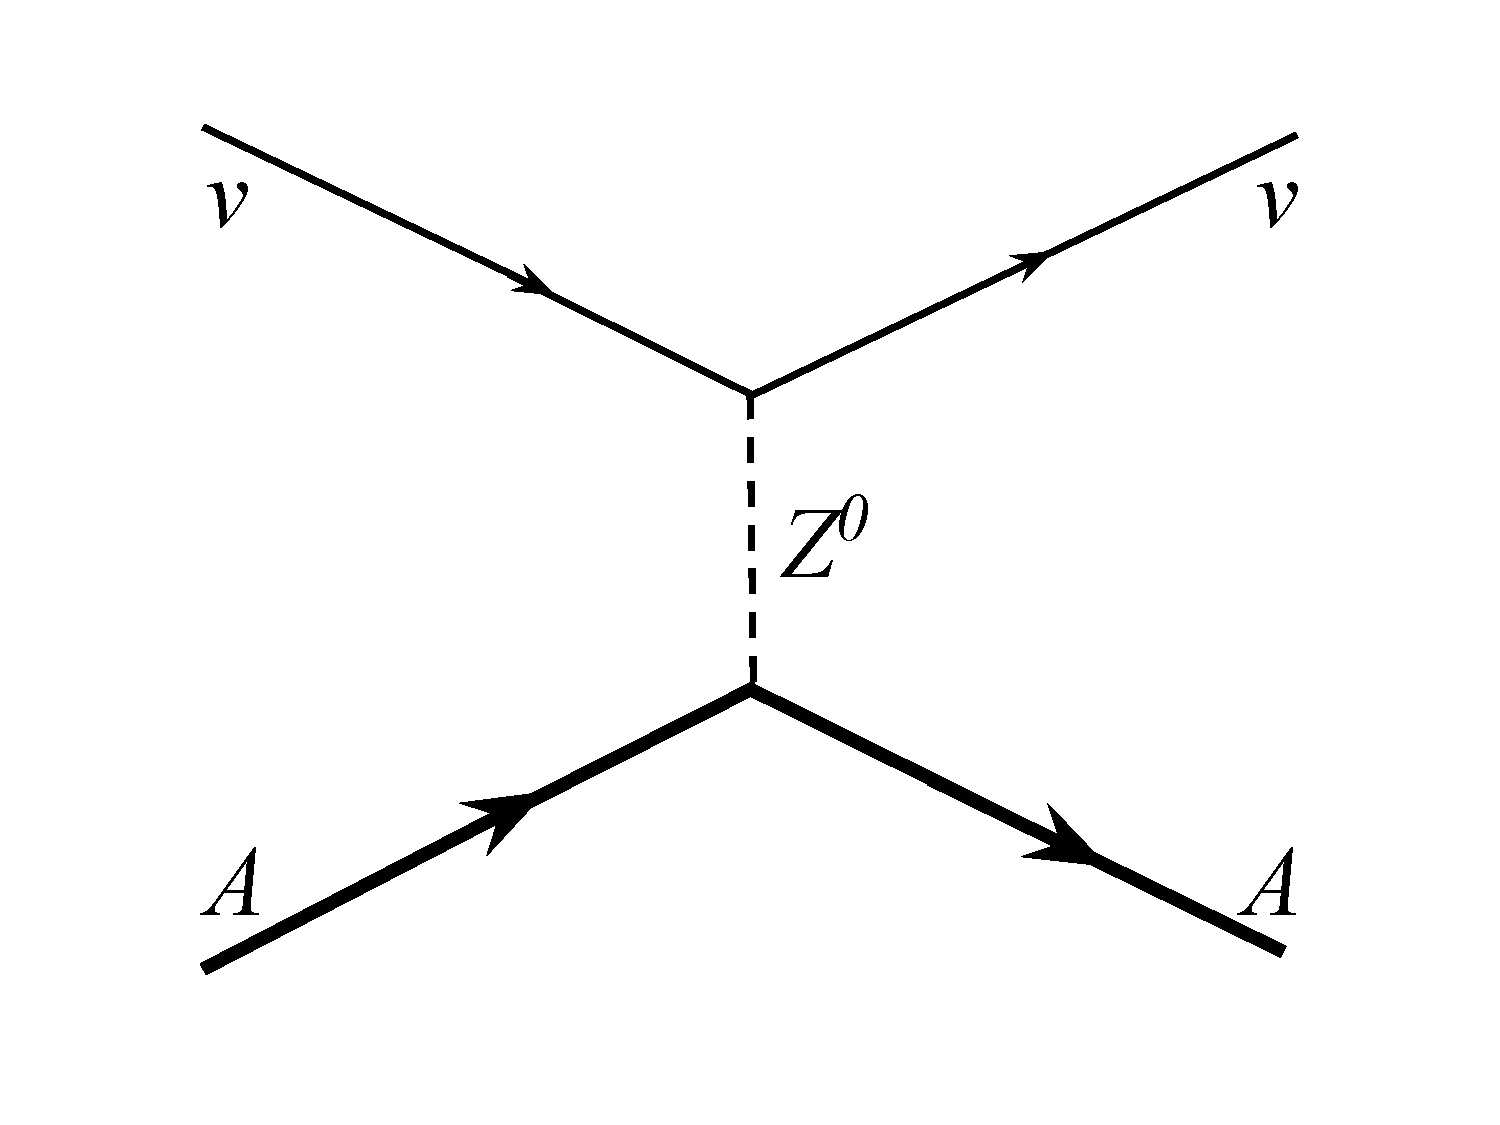
\includegraphics[width=0.6\linewidth]{images/cevns.pdf}}
	\caption{Схема когерентного рассеяния нейтрино на ядре}
	\label{ris:cevns}
\end{figure}
\par Дифференциальное сечение процесса представляется формулой \cite{cevns1, Lindner2017}:
	
\begin{equation}
\frac{d\sigma}{dE_r} = \frac{G_f^2}{4\pi} Q_w^2M\left(1-\frac{ME_r}{2E_\nu}\right)F^2(Q^2),
\end{equation}\\
	
	где $G_f$ --- константа Ферми;
	$Q_w=N-(1-4\sin^{2}\theta_w)Z$ --- слабый заряд для ядра с числом нуклонов $N$ и зарядом ядра $Z$;
	$F(Q^2)$ --- форм-фактор;
	$\theta_w$ --- угол смешивания слабого взаимодействия (угол Вайнберга).
	Используя значение угла можно показать, что сечение взаимодействия
	 $\sim N^2$:\\
	 
	$\sin^2(Q_w)\approx 0.22$ $\to Q_w\sim N \to \sigma \sim N^2$\\
	
	Полное сечение процесса приближённо равно:\\
	
	$\sigma \approx 0.4\cdot10^{-44}  N^2$(E$_\nu^2)$см$^{2}$/МэВ. \\
	\par
	Процесс УКРН имеет место при энергии нейтрино менее 50 МэВ, когда длина волны де Бройля для нейтрино не превосходит размеры ядра, и взаимодействие идет когерентно.
	Отметим, максимальная энергия ядра отдачи равна
\begin{equation}
    T_{max} = \frac{2E_{\nu}^{2}}{M+2E_{\nu}},
    \label{Tmax}
\end{equation}
то есть для большинства элементов энергия ядра отдачи очень мала --- порядка единиц-десятков кэВ на ядро. Таким образом возникают серьезные экспериментальные трудности при регистрации подобных процессов.

Впервые процесс УКРН был зарегистрирован коллаборацией COHERENT в 2017 году на детекторе CsI[Na]~\cite{COHERENT:2017ipa}. Через несколько лет успех коллаборации был повторен и процесс был зарегистрирован на ядрах аргона \cite{PhysRevLett.126.012002}. На данный момент в мире существует более 10 экспериментов по исследованию УКРН. Среди них есть эксперименты как на ускорителях \cite{COHERENT:2018gft}, так и на реакторах \cite{Belov_2015, Aguilar-Arevalo_2016, ricochet, Buck_2020, Singh:2016glu, Strauss_2020, Chaudhuri:2022pqk}. 

\textbf{Раздел 1.2} посвящен двухфазному методу регистрации частиц. В 1970 году Б.А. Долгошеиным был предложен~\cite{Dolgoshein} метод, основанный на использовании двух фаз рабочего вещества. Схема работы метода изображена на рисунке \ref{img:twophase}.
\begin{figure}[h]
	\center{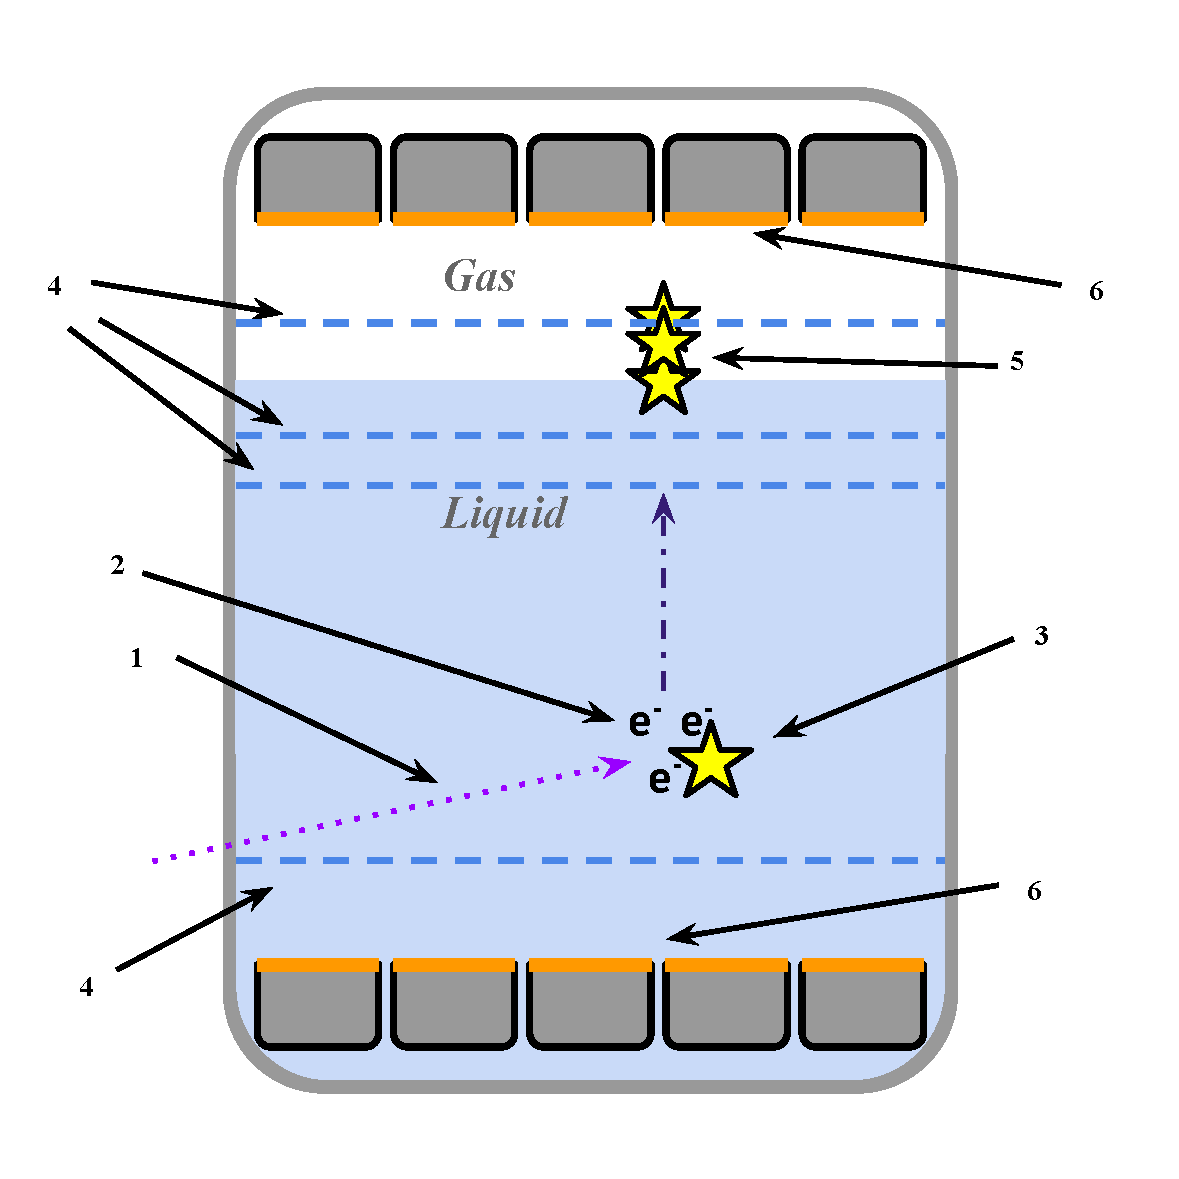
\includegraphics[width=0.7\linewidth]{images/twophasedetector.pdf}}
	\caption[Схема работы двухфазного детектора.] {Схема работы двухфазного детектора. 1 -- трек ионизирующей частицы; 2 -- электроны ионизации, возникшие в результате взаимодействия; 3 -- вспышка сцинтилляции (S1), возникшая в результате взаимодействия; 4 -- электроды-сетки, создающие напряжение; 5 -- электролюминесценция (S2) в электролюминесцентном зазоре; 6 -- матрицы из фотоумножителей}
	\label{img:twophase}
\end{figure}

Двухфазный метод регистрации частиц на данный момент широко используется в экспериментах по поиску темной материи~\cite{BOLOZDYNYA2015405}. Отличительной чертой всех экспериментов по исследованию темной материи явлется расположение глубоко под землей. Толща породы обеспечивала естественное экранирование от космических лучей. Детектор РЭД-100 раполагался на поверхности Земли, что потребовало модификации двухфазного метода регистрации с учетом повышенного фона от космических мюонов. 

\underline{\textbf{Вторая глава}} полностью посвящена эксперименту РЭД-100. В 2021-22 гг. на реакторе четвертого энергоблока Калининской АЭС был поставлен эксперимент РЭД-100 по исследованию УКРН ~\cite{The_RED100_Experiment}. Это один из немногих экспериментов, поставленных на промышленном реакторе. РЭД-100 был создан прицельно для измерения УКРН. Постановке эксперимента на Калининской АЭС предшествовал длительный подготовительный процесс в ЛЭЯФ НИЯУ МИФИ, включавший в себя наладку оборудования и инженерные запуски. 

\textbf{Раздел 2.1} посвящен устройству детектора РЭД-100. Схема детектора РЭД-100 приведена на рисунке \ref{img:detscheme}. Общий вес ксенона в системе РЭД-100 составляет около 200 кг, при этом вес непосредственно рабочего объема, участвующего в регистрации частиц -- 130 кг. В разделе приведено детальное описание газовой и криогенной систем детектора, системы полезадающих электродов-сеток, триггерной системы. 

\begin{figure}[ht!]	\center{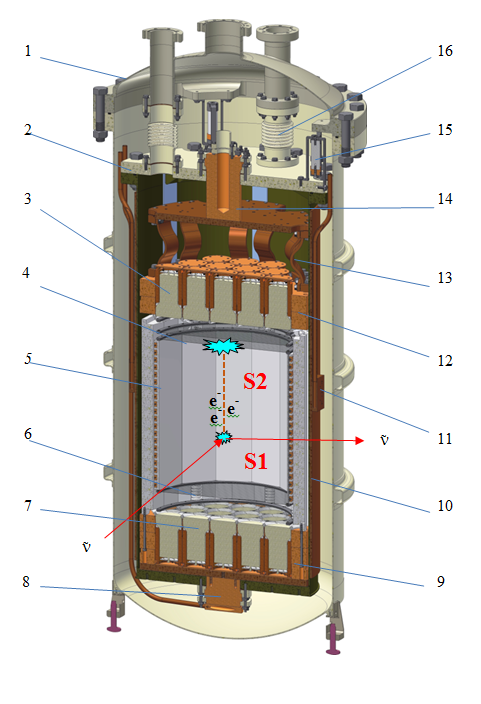
\includegraphics[width=0.5\linewidth]{images/red100.png}}
	\caption[Принцип работы и устройство детектора РЭД-100] {Принцип работы и устройство детектора РЭД-100. 1 --- внешний сосуд титанового криостата, 2 --- внутренний сосуд титанового криостата, 3 --- верхняя матрица из девятнадцати ФЭУ типа Hamamatsu R11410-20, 4 --- сетчатый анод и электронный затвор, 5 --- рабочий объем, окруженный тефлоновым отражателем со встроенными полезадающими электродами, 6 --- сетчатый катод, 7 --- нижняя матрица из девятнадцати ФЭУ, 8 --- нижний центральный теплосъемник с термосифоном, 9 --- медная обойма для нижней матрицы ФЭУ, 10 --- медный кожух холодного сосуда криостата, 11 --- один из двух боковых теплосъемников с термосифонами, 12 --- медная обойма верхней матрицы ФЭУ, 13 --- гибкий тепловой мост, 14 --- верхний центральный теплосъемник с медным диском, на котором конденсируется ксенон, 15 --- теплоизолирующий подвес, 16 --- сильфонная тепловая развязка для вывода кабелей; $e^-$ --- электроны ионизации, $\overline{\nu}$ --- антинейтрино, передающее энергию ядру отдачи, S1 --- сцинтилляционная вспышка, S2 --- электролюминесцентная вспышка.}
	\label{img:detscheme}
\end{figure}

Кроме того, в разделе описаны методы калибровки детектора РЭД-100, такие как:
\begin{itemize}
    \item LED-калибровка
    \item SE-данные (SE -- single electron)
    \item мюонные данные
    \item измерения с гамма-источниками
\end{itemize}
Также в разделе приводится описание основных источников внешнего и внутреннего фона в детекторе. В заключении раздела описан программный пакет RED-Offline, предназначенный для первичной обработки форм сигналов сцинтилляционных детекторов. В первичную обработку входят коррекция наводок, поиск нулевой линии, идентификация и параметризация импульсов. 

\textbf{Раздел 2.2} посвящен конфигурации установки при различных наборах данных. В работе рассматривается инженерный запуск детектора РЭД-100 в 2019 году и физический сеанс на Калининской АЭС в 2021-22 гг. В разделе приведены отличия в типах набираемых данных и конфигурациях пассивной защиты. 
Детектор РЭД-100 на Калининской АЭС располагался в 19 метрах снизу от реактора 4 энергоблока. В в качестве основной пассивной защиты от космических мюонов выступали бетонные перекрытия здания энергоблока. Далее конструкция детектора была помещена в мягкий бак из ПВХ диаметром 5 м, наполненный водой, что обеспечивало пассивную защиту от нейтронов толщиной 60 см. Для защиты от гамма фона вокруг детектора была выстроена конструкция из медных брусков толщиной 5 см. Данные набирались в периоды как с включенным, так и с выключенным реактором для сравнения спектров. 
Всего набирались шесть основных типов данных:
 \begin{enumerate}
     \item LED-калибровки
     \item Мюонные данные
     \item SE-данные
     \item Гамма-фон
     \item Гамма-калибровки
     \item УКРН-подобные данные
 \end{enumerate}
 Типы набранных во время инженерного сеанса в МИФИ данных совпадают с типами данных, набранных на КАЭС, за исключением УКРН-подобных данных. 
 Также в разделе приведены графики нейтронного и гамма фонов, измеренных на протяжении постановки эксперимента на КАЭС при помощи вспомогательных детекторов (NaI[Tl] и Bicron) (рисунок~\ref{img:gammaneutronbckg}).

 \begin{figure}[ht!]
  \begin{minipage}[ht]{0.49\linewidth}
    \center{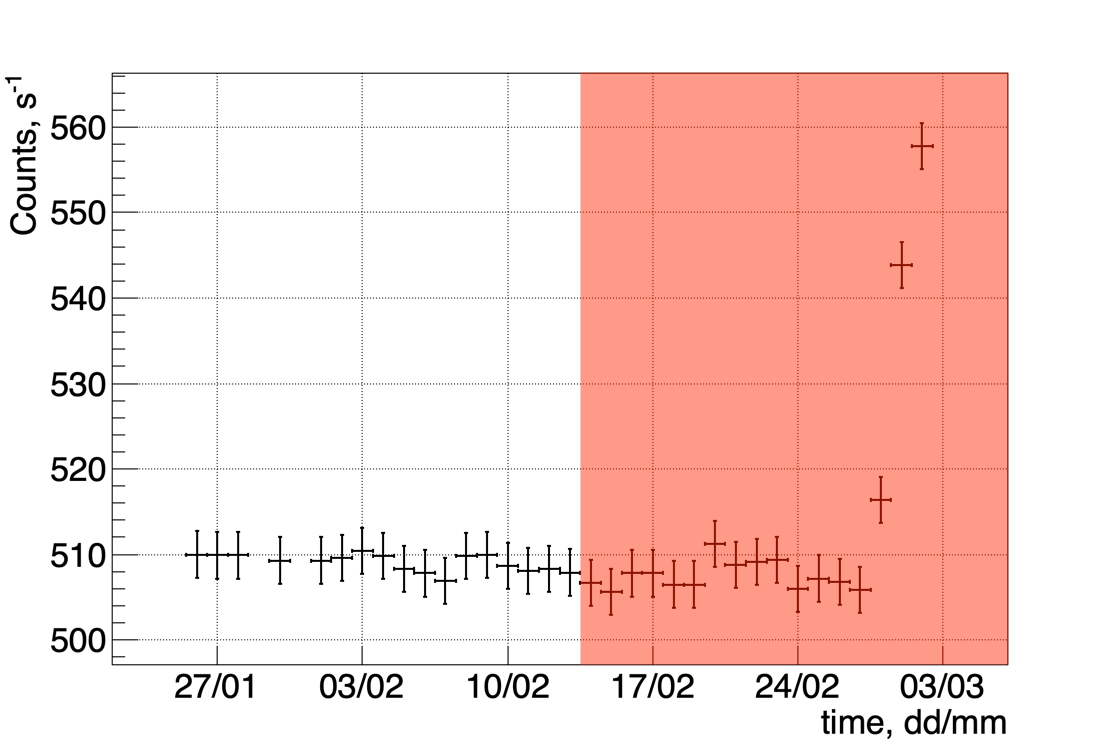
\includegraphics[width=1.0\linewidth]{images/NaI_count_rate_monitoring.png} \\ а)}
  \end{minipage}
  \hfill
  \begin{minipage}[ht]{0.49\linewidth}
    \center{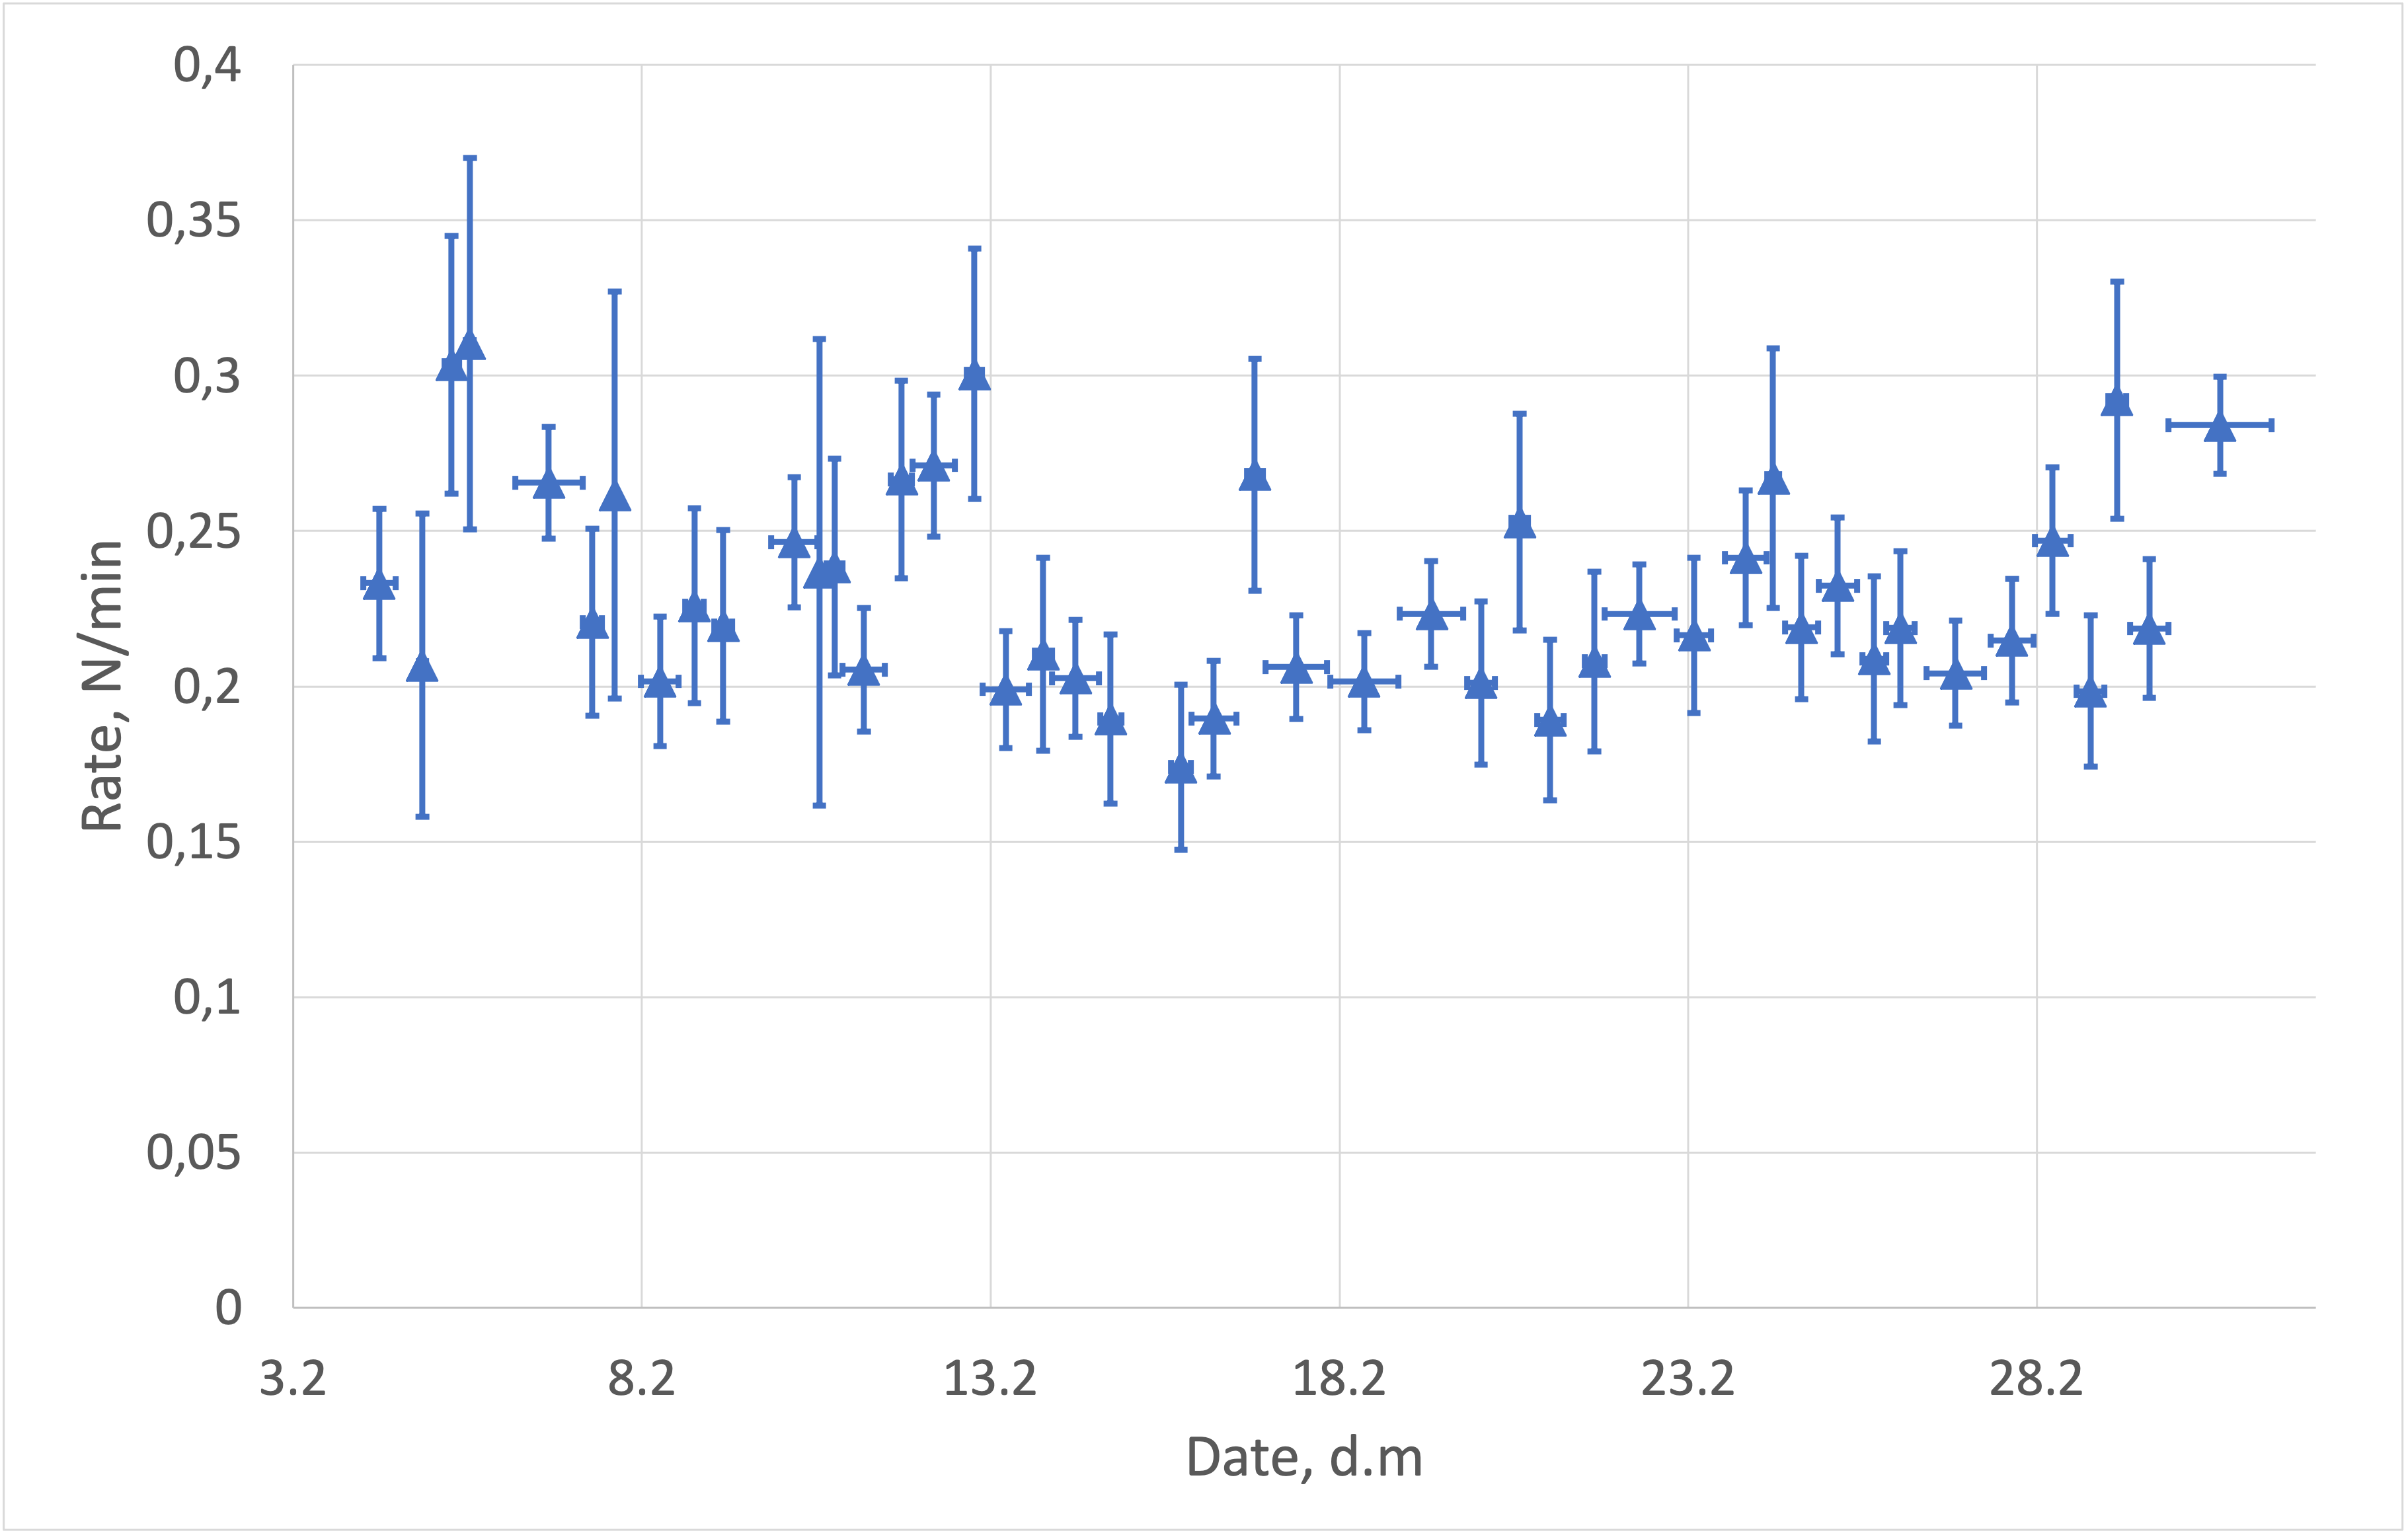
\includegraphics[width=1.0\linewidth]{images/neutrons_rate.png} \\ б)}
  \end{minipage}
  \caption[Графики изменения гамма и нейтронного фонов.]{а) График изменения гамма-фона (измерения суммировались за каждые 3 часа набора данных). б) График изменения нейтронного фона}
  \label{img:gammaneutronbckg}  
\end{figure}

 \textbf{Раздел 2.3} посвящен моделированию детектора РЭД-100. Приведено описание моделей детектора в трех программных пакетах (GEANT4, NEST, ANTS-2), а также описание моделирования временных разверток сигналов. 

 \underline{\textbf{Третья глава}} посвящена анализу калибровочных данных детектора РЭД-100.  
 
 \textbf{Раздел 3.1} посвящен калибровке мюонами. При дрейфе в ксеноне электроны ионизации претерпевают потери, связанные с захватом их примесями. Как известно, процесс таких потерь описывается экспоненциальной функцией. Для измерения времени жизни мюонные сигналы, записанные в специальном режиме работы детектора, фитировались функцией $ f(t) = A\cdot exp(-\frac{t}{\tau})$, где $\tau$ -- среднее времени
жизни электронов до захвата $\tau$, за которое количество дрейфующих электронов ионизации уменьшается в e раз. Пример усредненного сигнала и его фитирования приведен на рисунке \ref{img:muonsignal}. Усреднение сигнала проводилось путем суммирования большого количества одиночных сигналов.
\begin{figure}[ht!]	\center{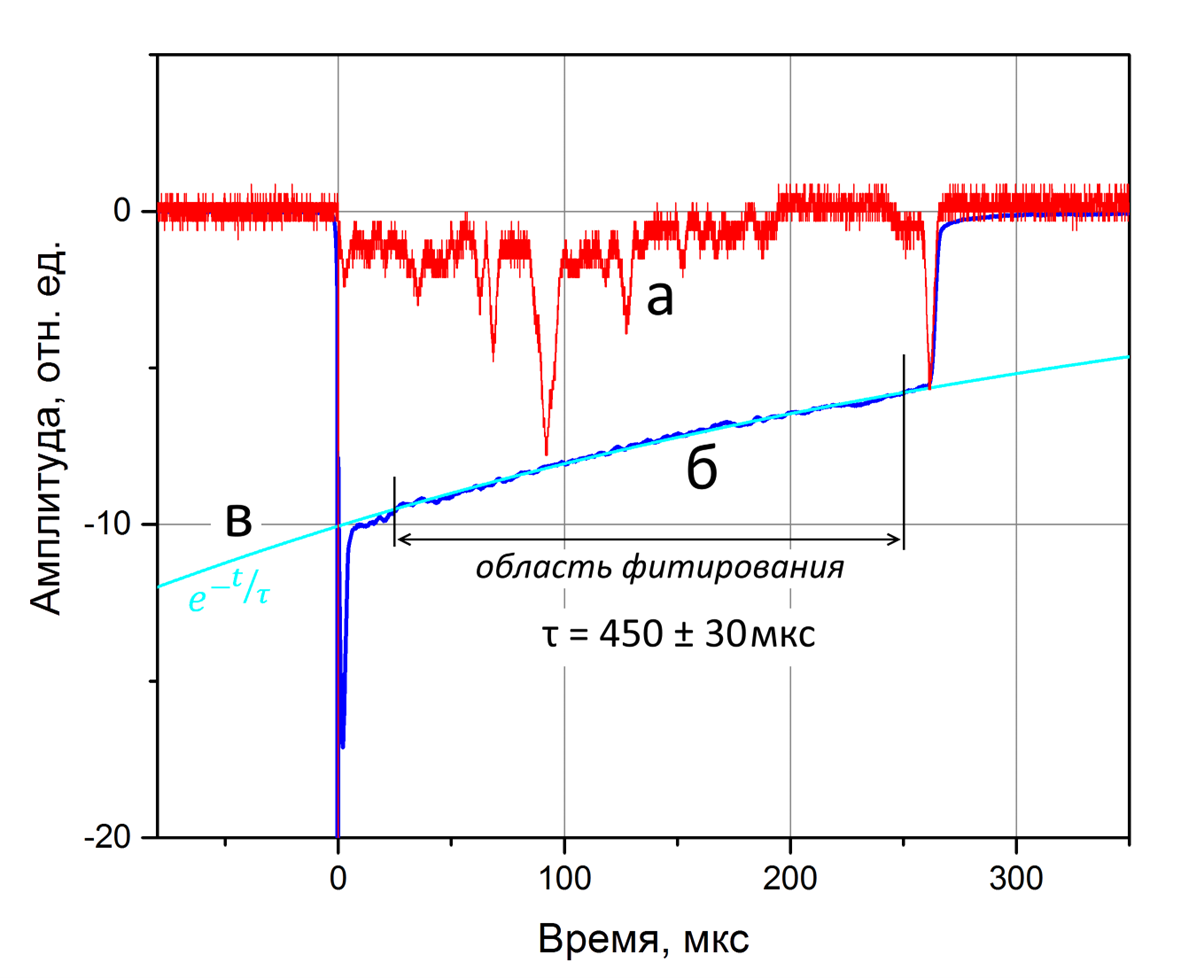
\includegraphics[width=0.8\linewidth]{images/Graph41_labels.png}}
	\caption[Пример определения времени жизни электронов ионизации до захвата электроотрицательными примесями в жидком ксеноне.]{а) — типичный мюонный сигнал, б) — сигнал, усреднённый по 10 000 событий, в — экспоненциально спадающая функция, аппроксимирующая «ступеньку» усреднённого сигнала.}
	\label{img:muonsignal}
\end{figure}

Эволюция времени жизни в течение сеанса показана
на рисунках \ref{img:lt2019}, \ref{img:lt2022}

\begin{figure}[ht!]	\center{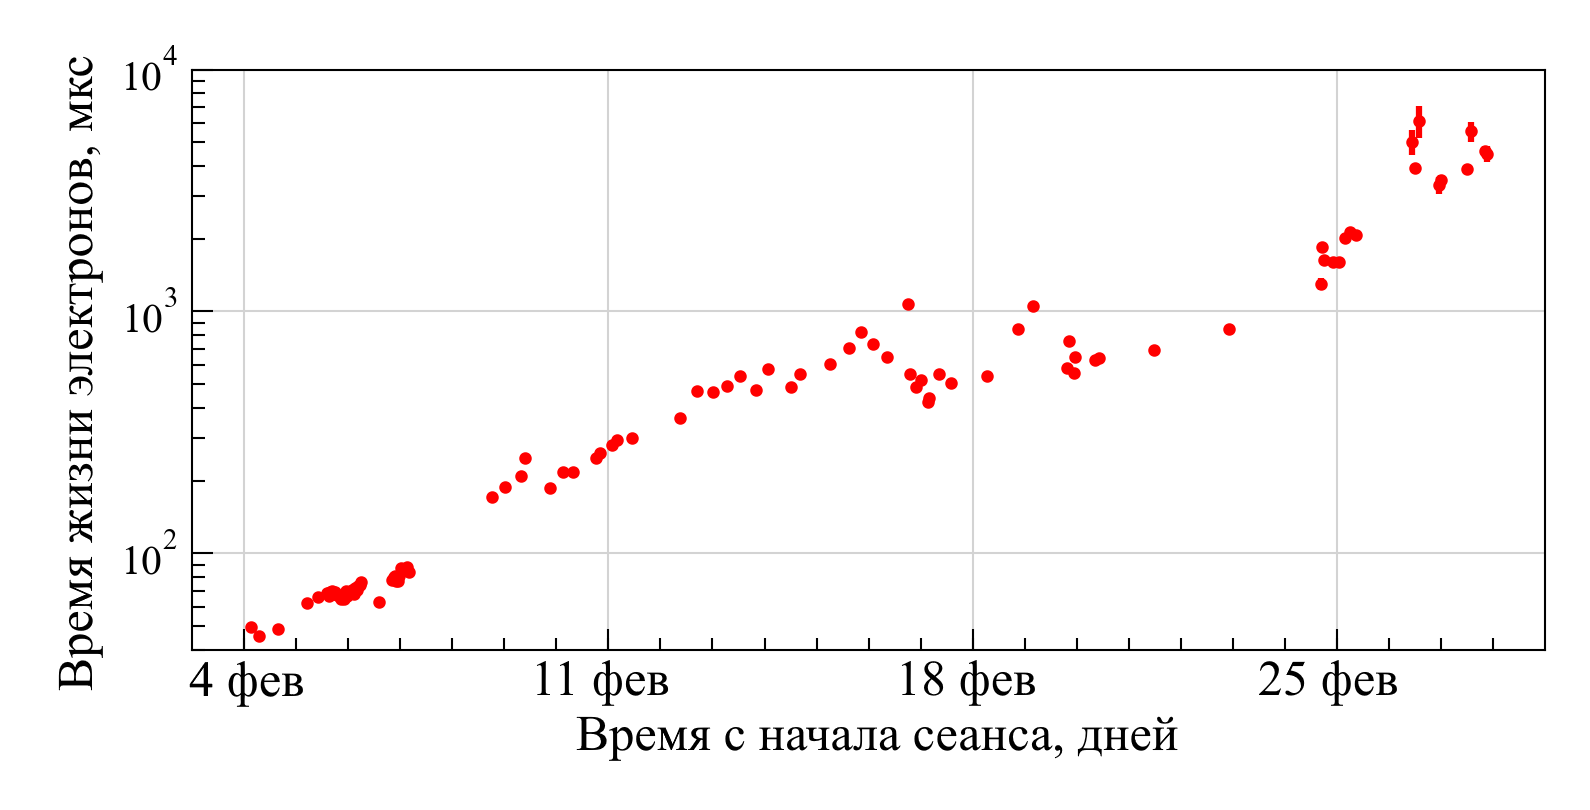
\includegraphics[width=0.8\linewidth]{images/RED100. Graph. e_lifetime_2019_published_RU.png}}
	\caption{Динамика изменения времени жизни электронов в детекторе РЭД-100 в течение инженерного сеанса 2019 года}
	\label{img:lt2019}
\end{figure}

\begin{figure}[ht!]	\center{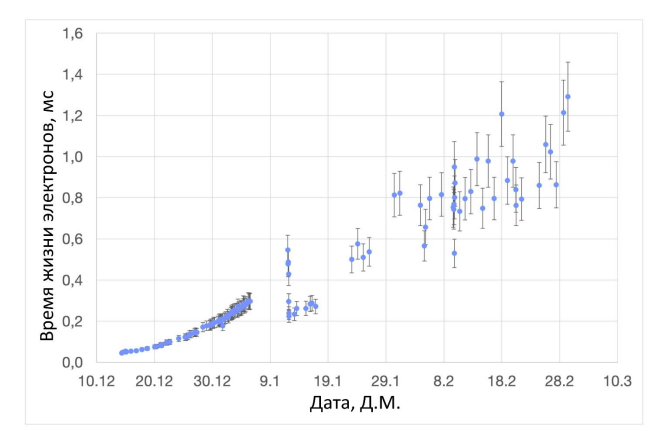
\includegraphics[width=0.8\linewidth]{images/lifetime2022.png}}
	\caption{Динамика изменения времени жизни электронов в детекторе РЭД-100 в течение сеанса на КАЭС 2022 года}
	\label{img:lt2022}
\end{figure}

В \textbf{разделе 3.2} описывается LED-калибровка, необходимая для определения среднего заряда SPE (single photo-electron) для каждого ФЭУ. После обработки данных пакетом REDOffline, из обнаруженных импульсов отбирались импульсы с амплитудой и длительностью больше пороговых. Далее распределение площадей отобранных импульсов фитировалось суммой экспоненциальной функции и распределения Гаусса, и исходя из параметров полученного распределения Гаусса вычислялся средний заряд SPE для каждого ФЭУ. Далее полученные значения использовались для перевода площадей импульсов из В$\cdot$c в единицы SPE.

\textbf{Раздел 3.3} посвящен анализу измерений с гамма-источниками. В 2019 году в качестве калибровочных источников использовались $^{60}$Co и $^{22}$Na, в 2021-22 -- $^{60}$Co и $^{137}$Cs. 

Гамма-кванты дают световыход в детекторе, достаточно большой для того, чтобы в каждом ФЭУ был ощутимый световой сигнал. Поэтому для анализа применяется суммарная форма сигнала, в которой импульсы от физических сигналов в разных ФЭУ будут складываться, а совпадений случайных импульсов с таковыми в других ФЭУ не будет. В разделе описан алгоритм кластеризации, позволяющий отбирать S1 и S2, соответствующие подобным событиям.

После кластеризации на события накладывались дополнительные отборы по глубине и по количеству S1 и S2 в каждом событии (строго по одной вспышке каждого вида). В разделе подробно описаны методы восстановления координат S2 в плоскости XY и энергии событий на основе LRF (light response functions). Кроме того, описан итеративный процесс получения данных функций. Восстановление координат и энергии позволяет существенно уменьшить зависимость светосбора от радиуса. 

В двухфазных детекторах присутствует антикорреляция между S1 и S2, поэтому в качестве энергии рассматривалась линейная комбинация сцинтилляции и электролюминесценции. Также для улучшения соотношения сигнал/шум на события были наложены дополнительные отборы по восстановленному радиусу (175 мм для сеанса в МИФИ и 130 мм для сеанса на КАЭС). Калибровочные графики для двух сеансов набора данных приведены на рисунках~\ref{img:calibplot2019},~\ref{img:calibr2022}, а энергетическое разрешение и положения пиков -- в таблицах~\ref{tab:resolution2019}~и~\ref{tab:resolution2022}. Различия в энергетическом разрешении связаны с различными отборами в двух сеансах и методами фитирования спектров.

\begin{figure}[ht]
\center{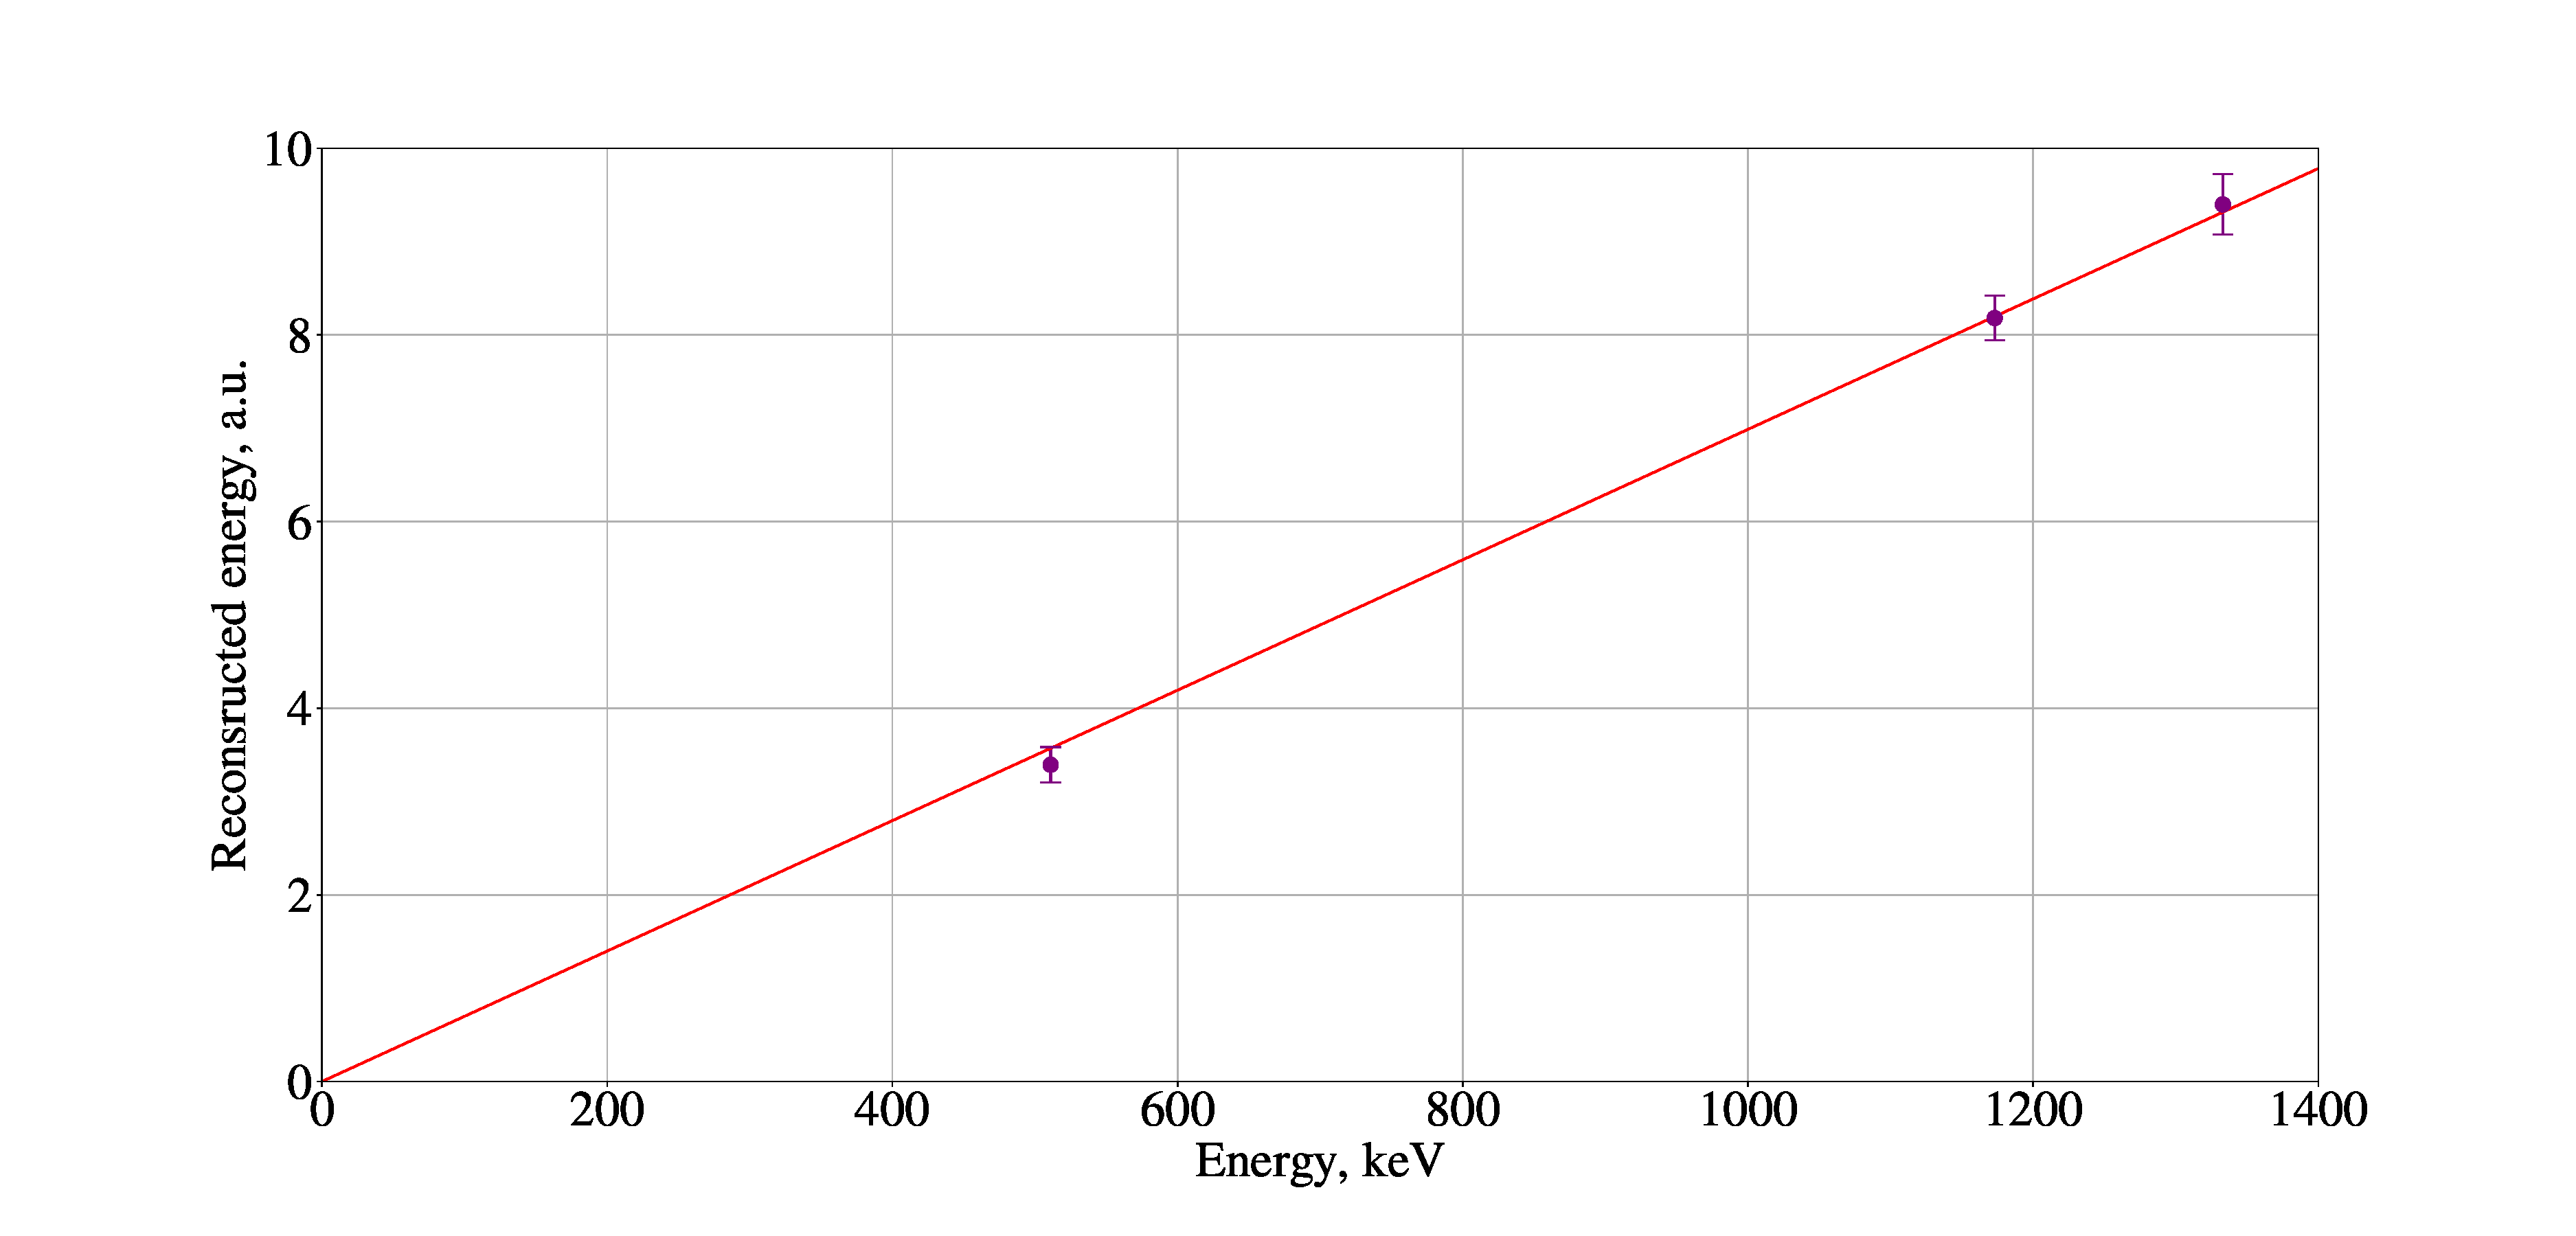
\includegraphics[width=1\linewidth]{images/calibr.pdf}}
  \caption{Калибровочный график для инженерного сеанса 2019 года.}
  \label{img:calibplot2019}  
\end{figure}

\begin{table}[ht]
    \centering
        \caption{Положения пиков и энергетическое разрешение}
\begin{tabular}{|c|c|c|c|}
\hline
    Энергия, кэВ & Положение пика, кэВ & ($\sigma/E$), \% & FWHM/E,  \%\\
    \hline
    511 & 486$\pm$29 & 5.5$\pm$0.1 & 12.9$\pm$0.2\\
    \hline
    1173 & 1171$\pm$34 & 5.4$\pm$0.1 & 12.7$\pm$0.3\\
    \hline
    1333 & 1345$\pm$46 & 4.8$\pm$0.2 & 11.3$\pm$0.4\\
    \hline
\end{tabular}
    \label{tab:resolution2019}
\end{table}

\begin{figure}[ht]
\center{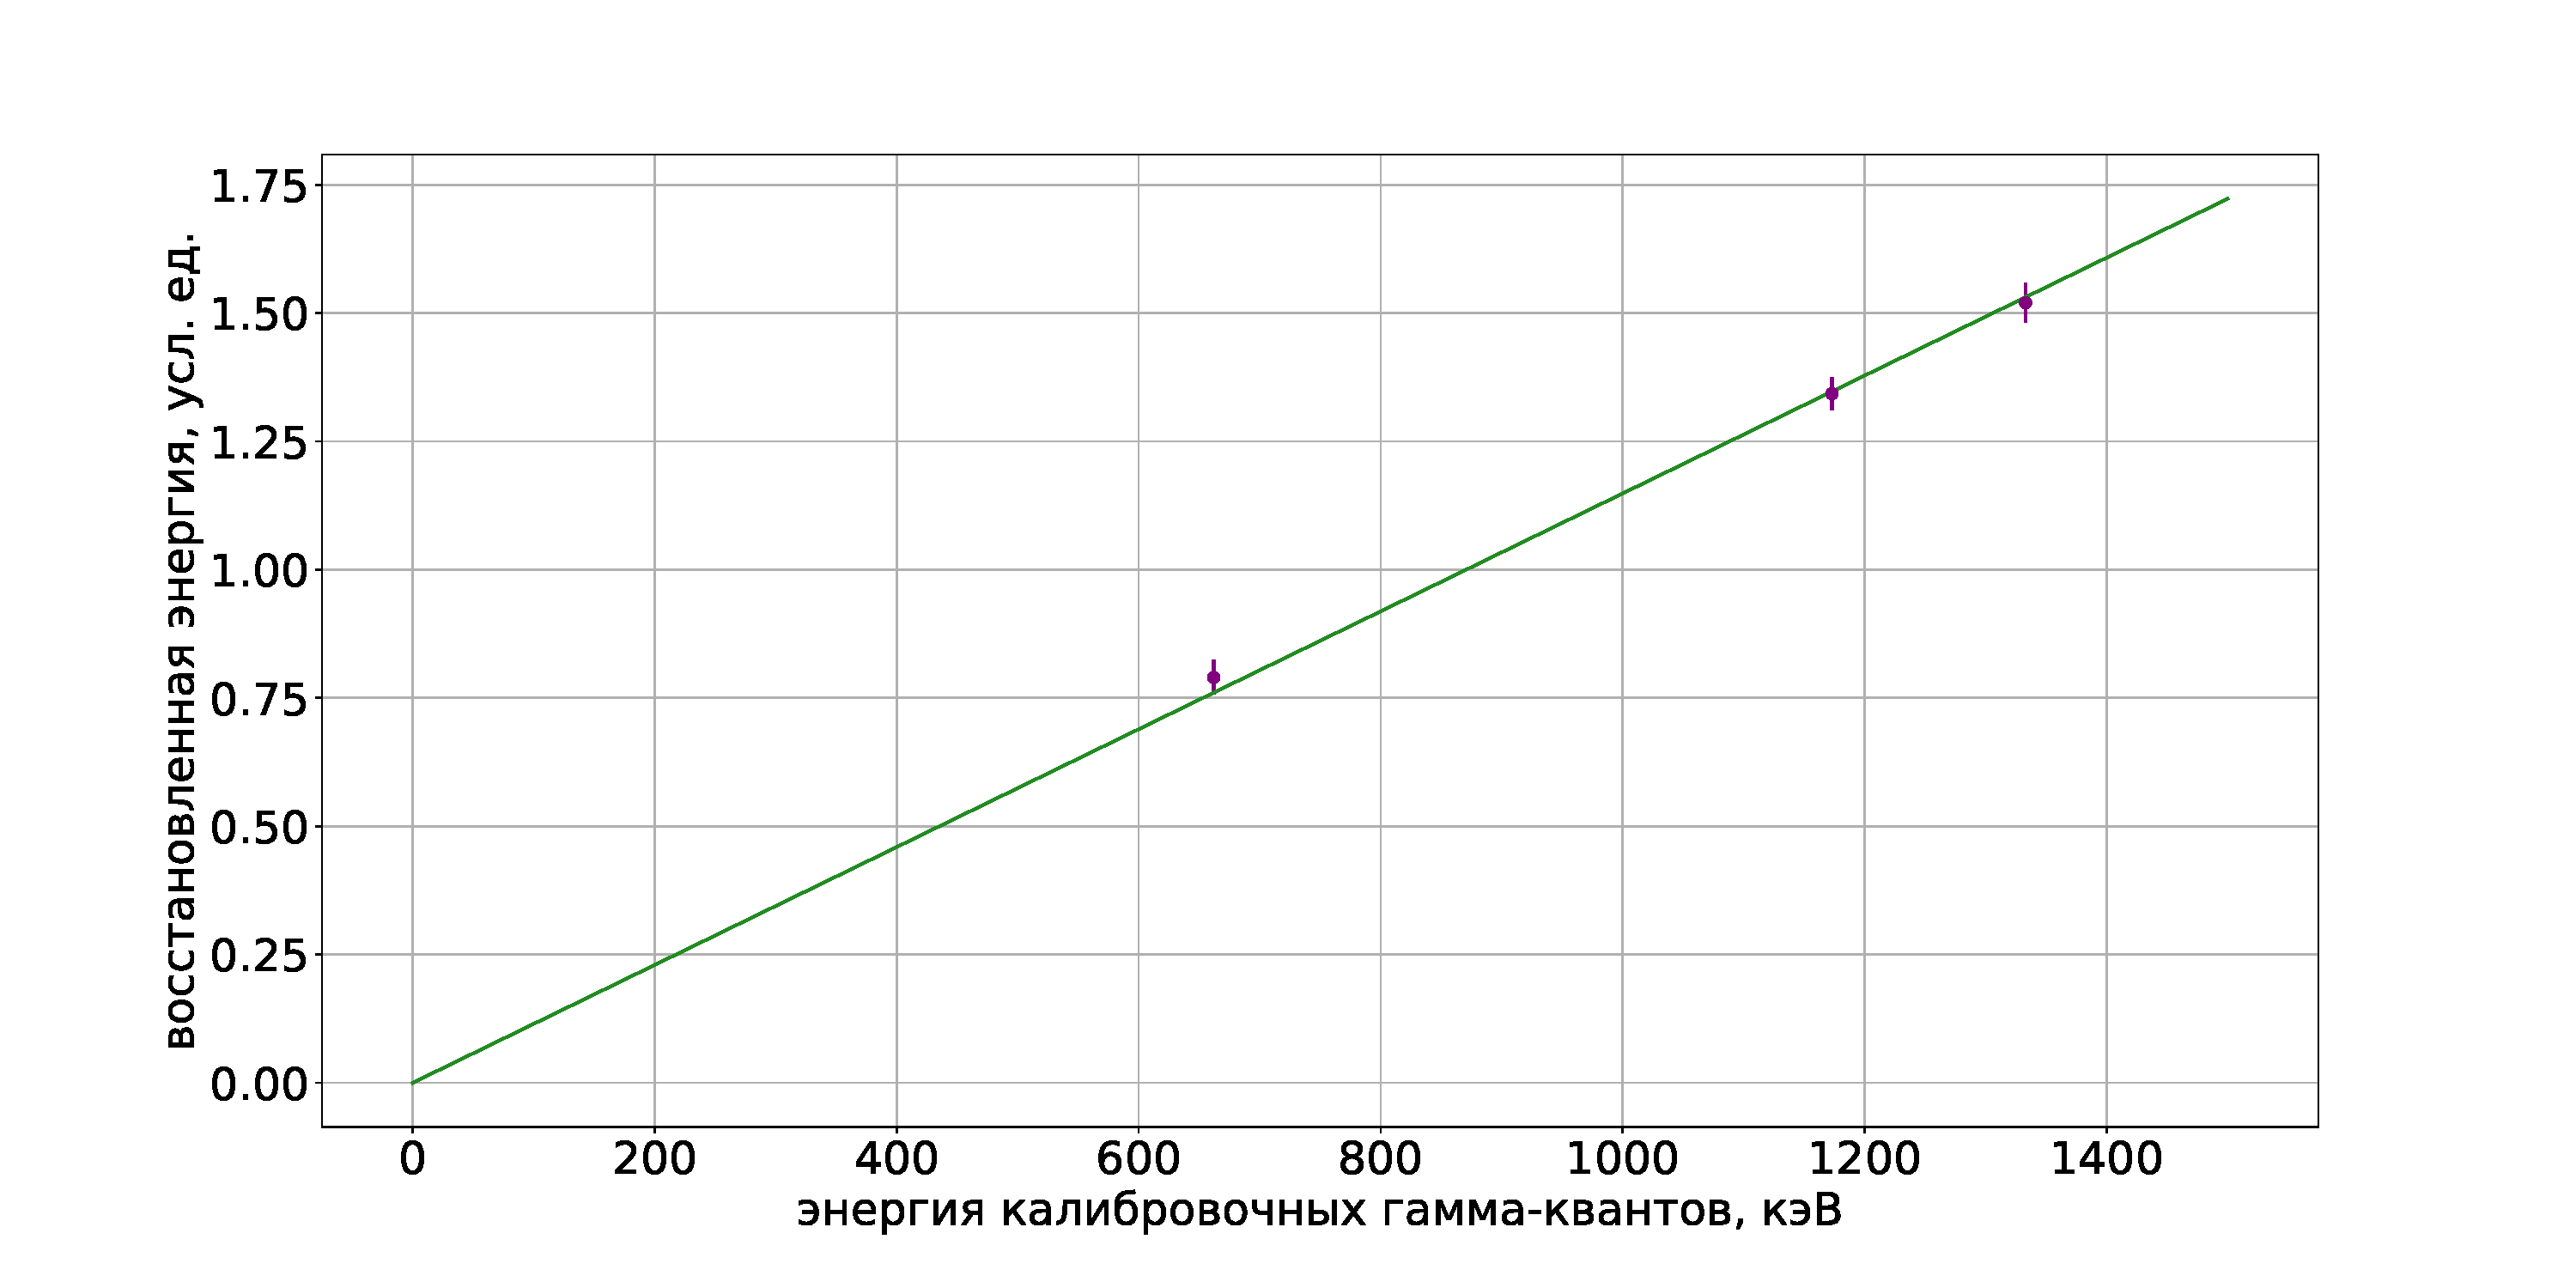
\includegraphics[width=1\linewidth]{images/calibr2022.pdf}}
  \caption{Калибровочный график для сеанса на КАЭС}
  \label{img:calibr2022}  
\end{figure}

\begin{table}[ht]
    \centering
        \caption{Положения пиков и энергетическое разрешение (сеанс на КАЭС)}
\begin{tabular}{|c|c|c|c|}
\hline
    Энергия, кэВ & Положение пика, кэВ & ($\sigma/E$), \% & FWHM/E,  \%\\
    \hline
    662 & 688$\pm$29 & 8.4 & 19.6\\
    \hline
    1173 & 1169$\pm$27 & 3.7 & 8.7\\
    \hline
    1333 & 1323$\pm$33 & 3.9 & 9.2\\
    \hline
\end{tabular}    
\label{tab:resolution2022}
\end{table}

\textbf{Раздел 3.4} посвящен SE-калибровкам. Сигналы от одиночных электронов ионизации представляют собой кластеры из равномерно распределенных по времени внутри кластера однофотоэлектронных импульсов. Как уже было упомянуто, SE-данные предсталяют собой формы сигналов в случайные моменты времени. Данные формы сигналов могут содержать как и искомые сигналы, так и совершенно разные события, а также случайные импульсы. Для отбора кластеров импульсов, соответствующих сигналам от одиночных электронов ионизации был применен следующий алгоритм:
\begin{enumerate}
    \itemОтбирались импульсы с амплитудой больше пороговой. Пороговые значения вычислялись как $\mu-2\sigma$, где $\mu$ и $\sigma$ -- параметры фита однофотоэлектронного спектра в соответствующем канале.
    \itemОтбирались такие последовательности импульсов, чтобы между любыми двумя из них расстояние было не больше $\Delta T$=500~нс. Величина $\Delta T$ подбиралась экспериментально исходя из знания о том, что длительность кластера, соответствующего электролюминесценции, составляет~$\approx$2~мкс. 
\end{enumerate}

Распределение SE-событий по длительности представлено на рисунке~\ref{img:seduration}. Как и во время сеанса на КАЭС, так и во время инженерного сеанса наблюдались события длительностью существенно меньшей, чем средняя длительность электролюминесценции. Данные события на графиках, представленных на рисунке~\ref{img:seduration}, составляют пик слева от основного. Такие "короткие" события возникают, если электролюминесценция происходит с самого края детектора, где электролюминесцентный зазор ограничен кольцом-держателем сетки. Для дальнейшего анализа данные события были отброшены. Границы отбора по длительности показаны на рисунке~\ref{img:seduration} красными линиями. Распределения суммарного светосбора по данным верхней матрицы для SE-данных представлены на рисунке~\ref{img:sespesp}.
\begin{figure}[ht]
  \begin{minipage}[ht]{0.49\linewidth}    \center{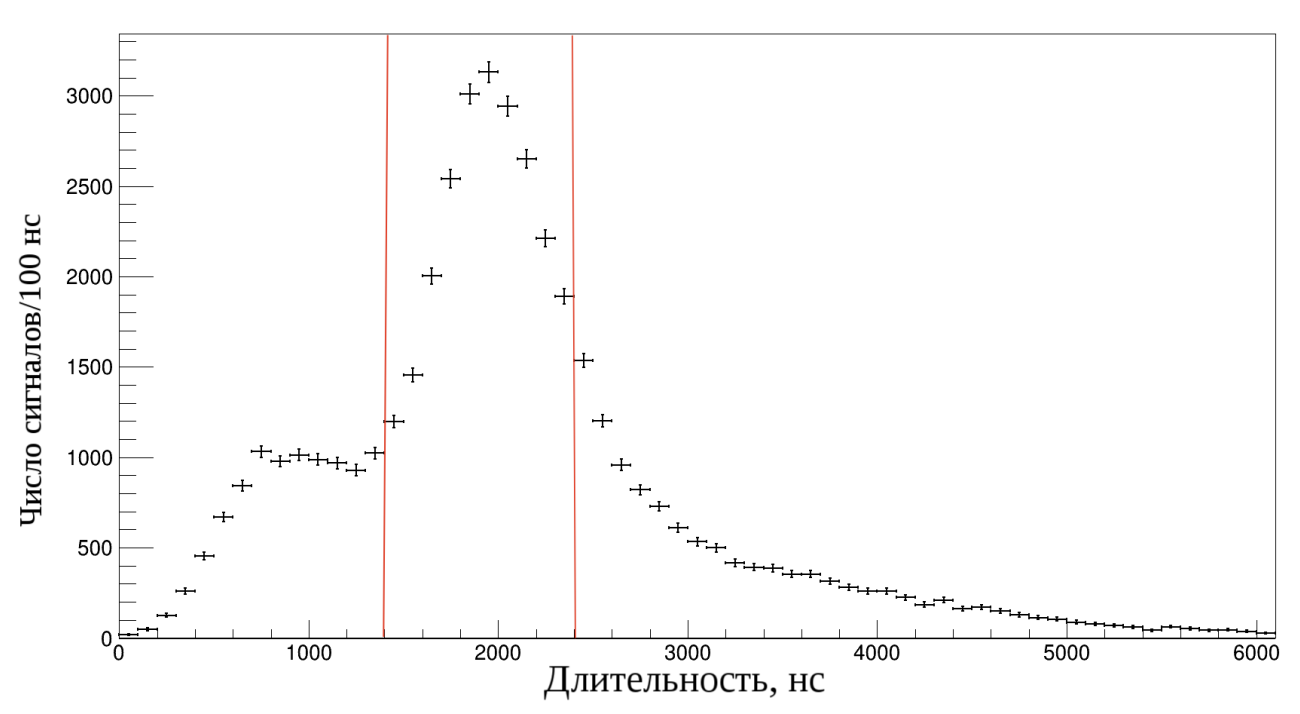
\includegraphics[width=1.0\linewidth]{images/seduration2019.png} \\ а)}
  \end{minipage}
  \hfill
  \begin{minipage}[ht]{0.49\linewidth}  \center{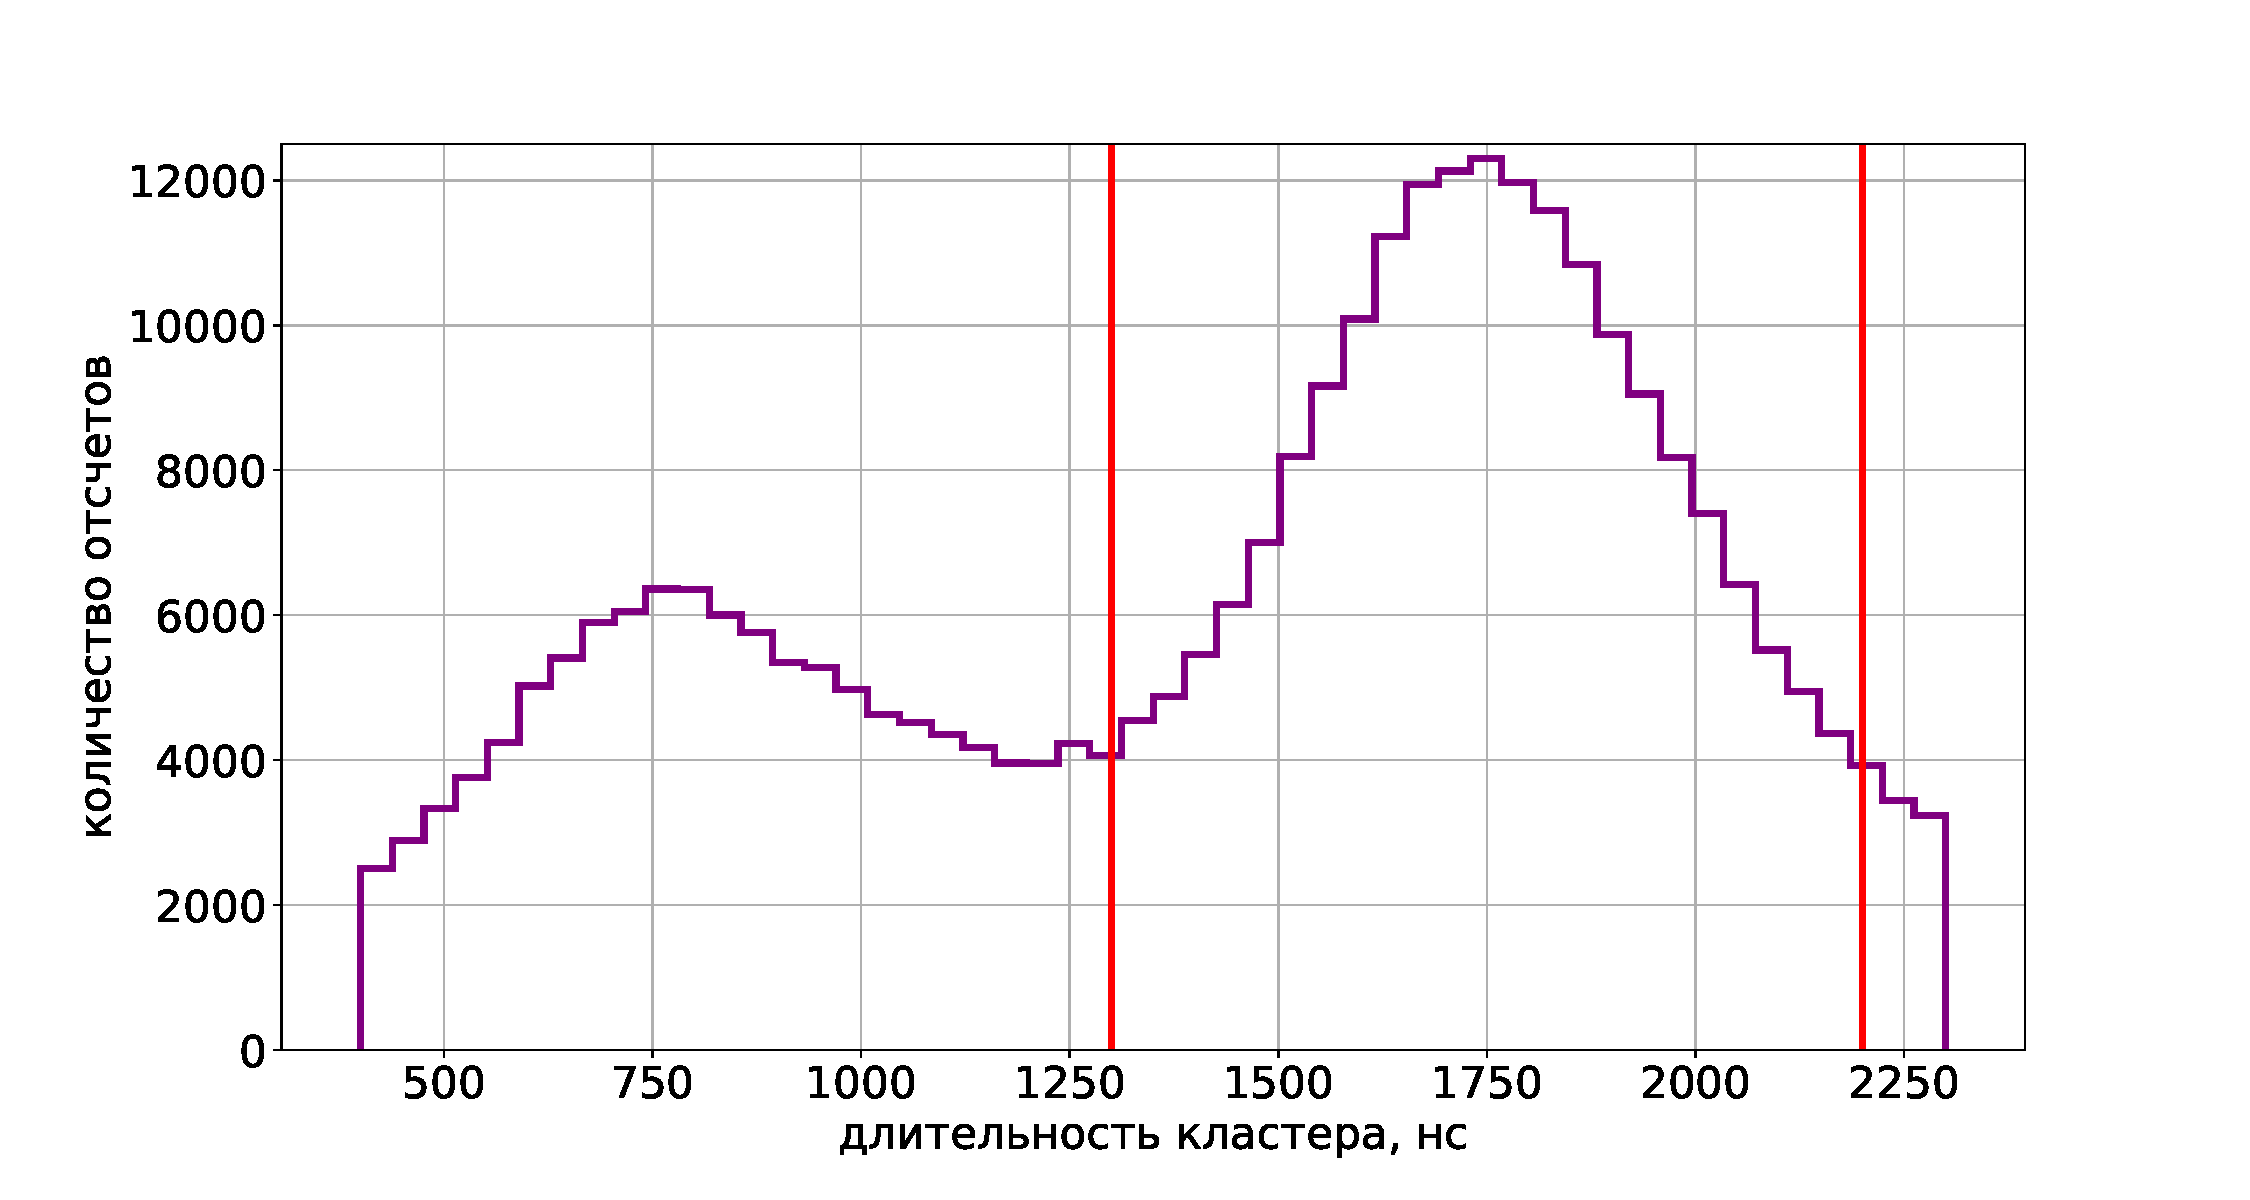
\includegraphics[width=1.0\linewidth]{images/seduration2022.pdf} \\ б)}
  \end{minipage}
  \caption{Распределение событий по длительности для инженерного сеанса (слева) и сеанса на КАЭС (справа)}
  \label{img:seduration}  
\end{figure}

\begin{figure}[ht]
  \begin{minipage}[ht]{0.49\linewidth}    \center{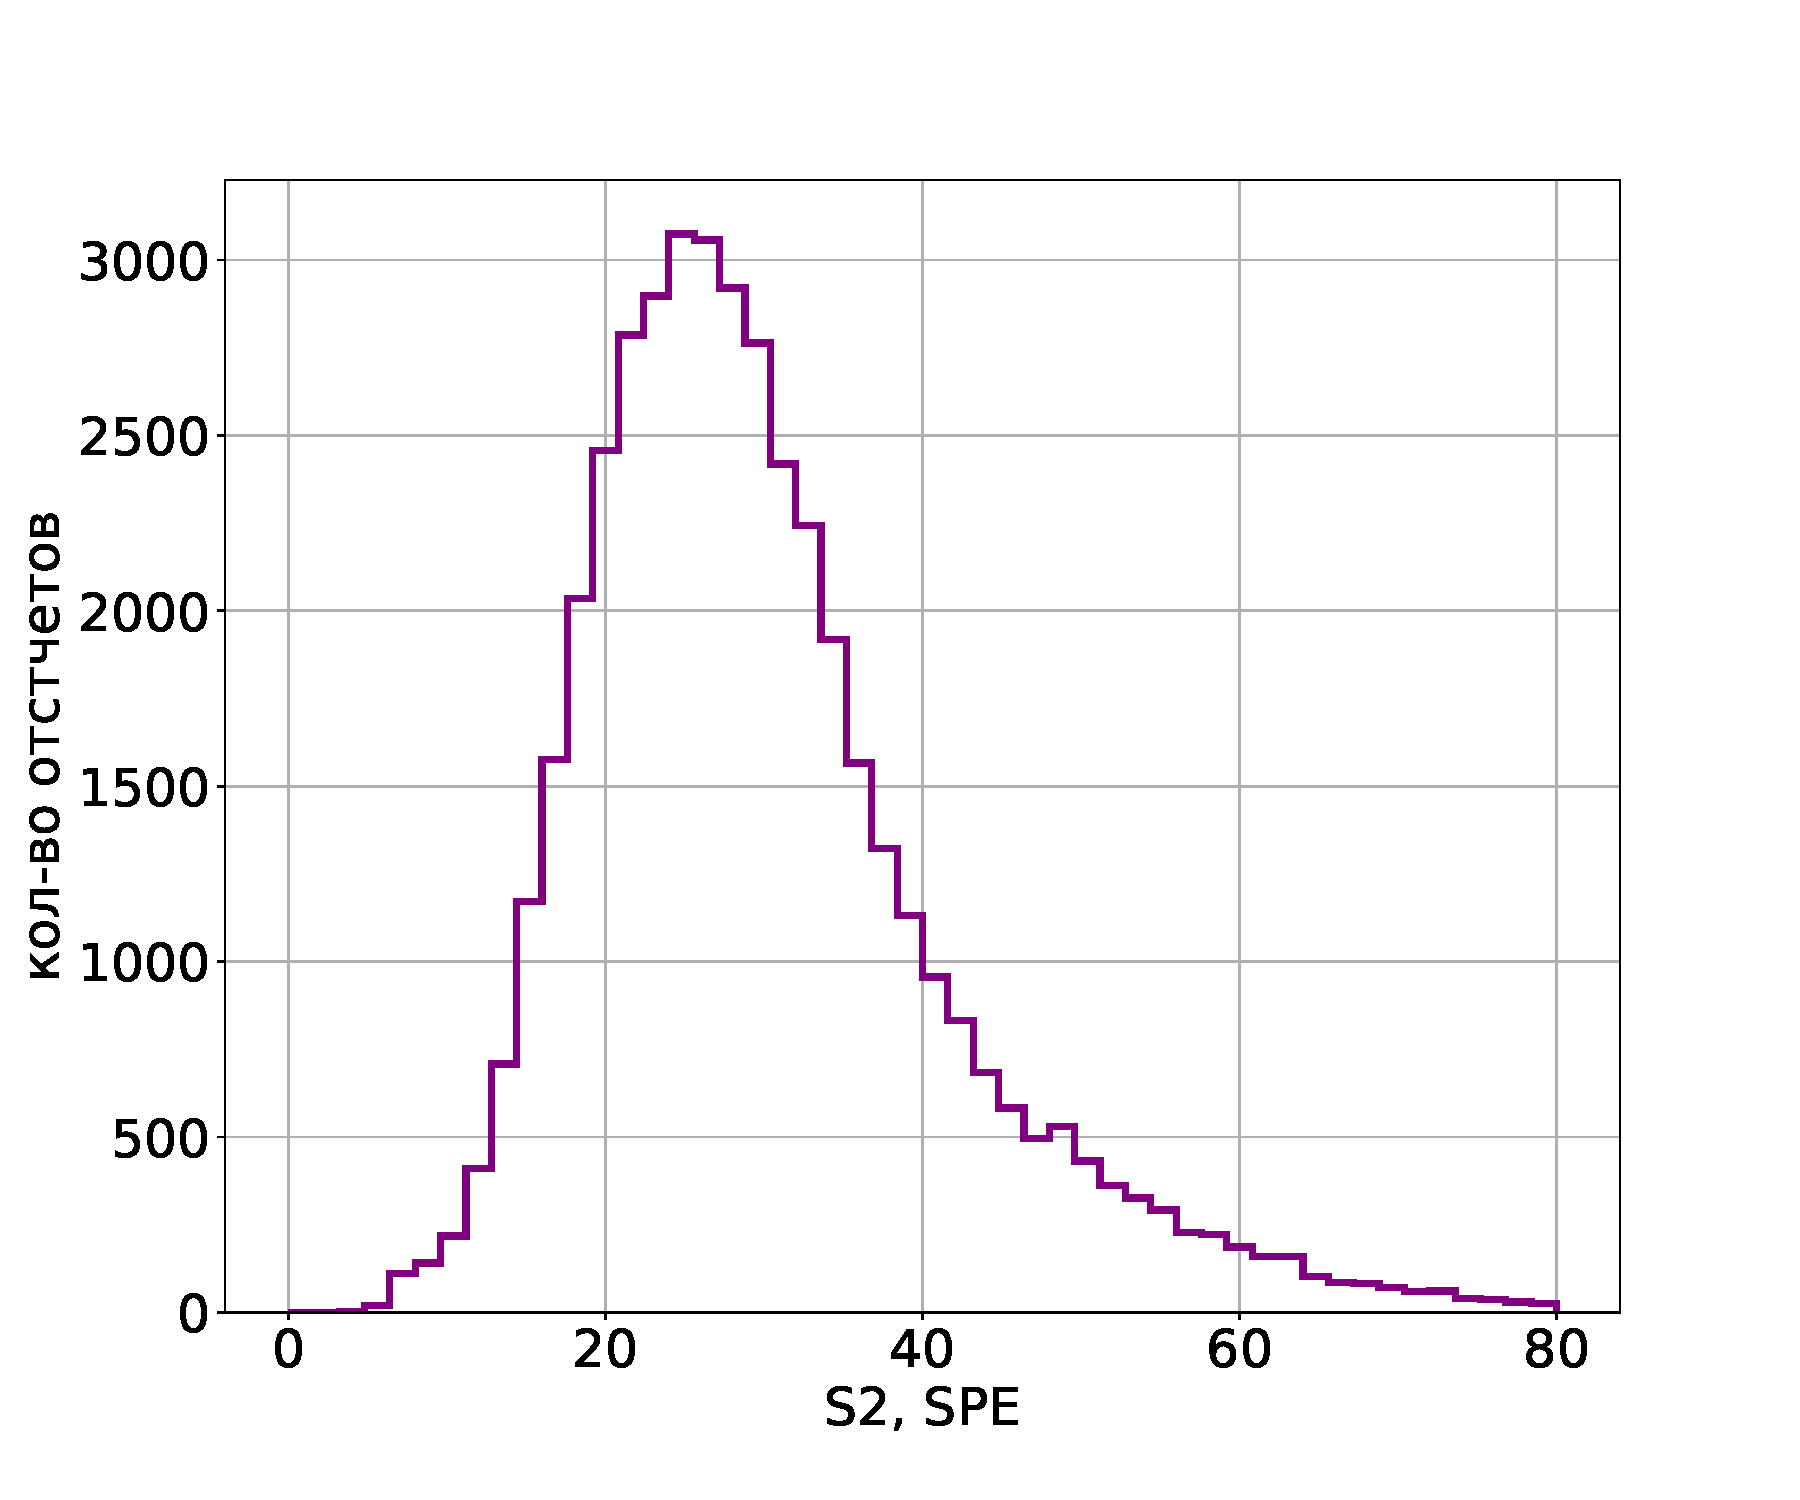
\includegraphics[width=1.0\linewidth]{images/se2019sp.pdf} \\ а)}
  \end{minipage}
  \hfill
  \begin{minipage}[ht]{0.49\linewidth}  \center{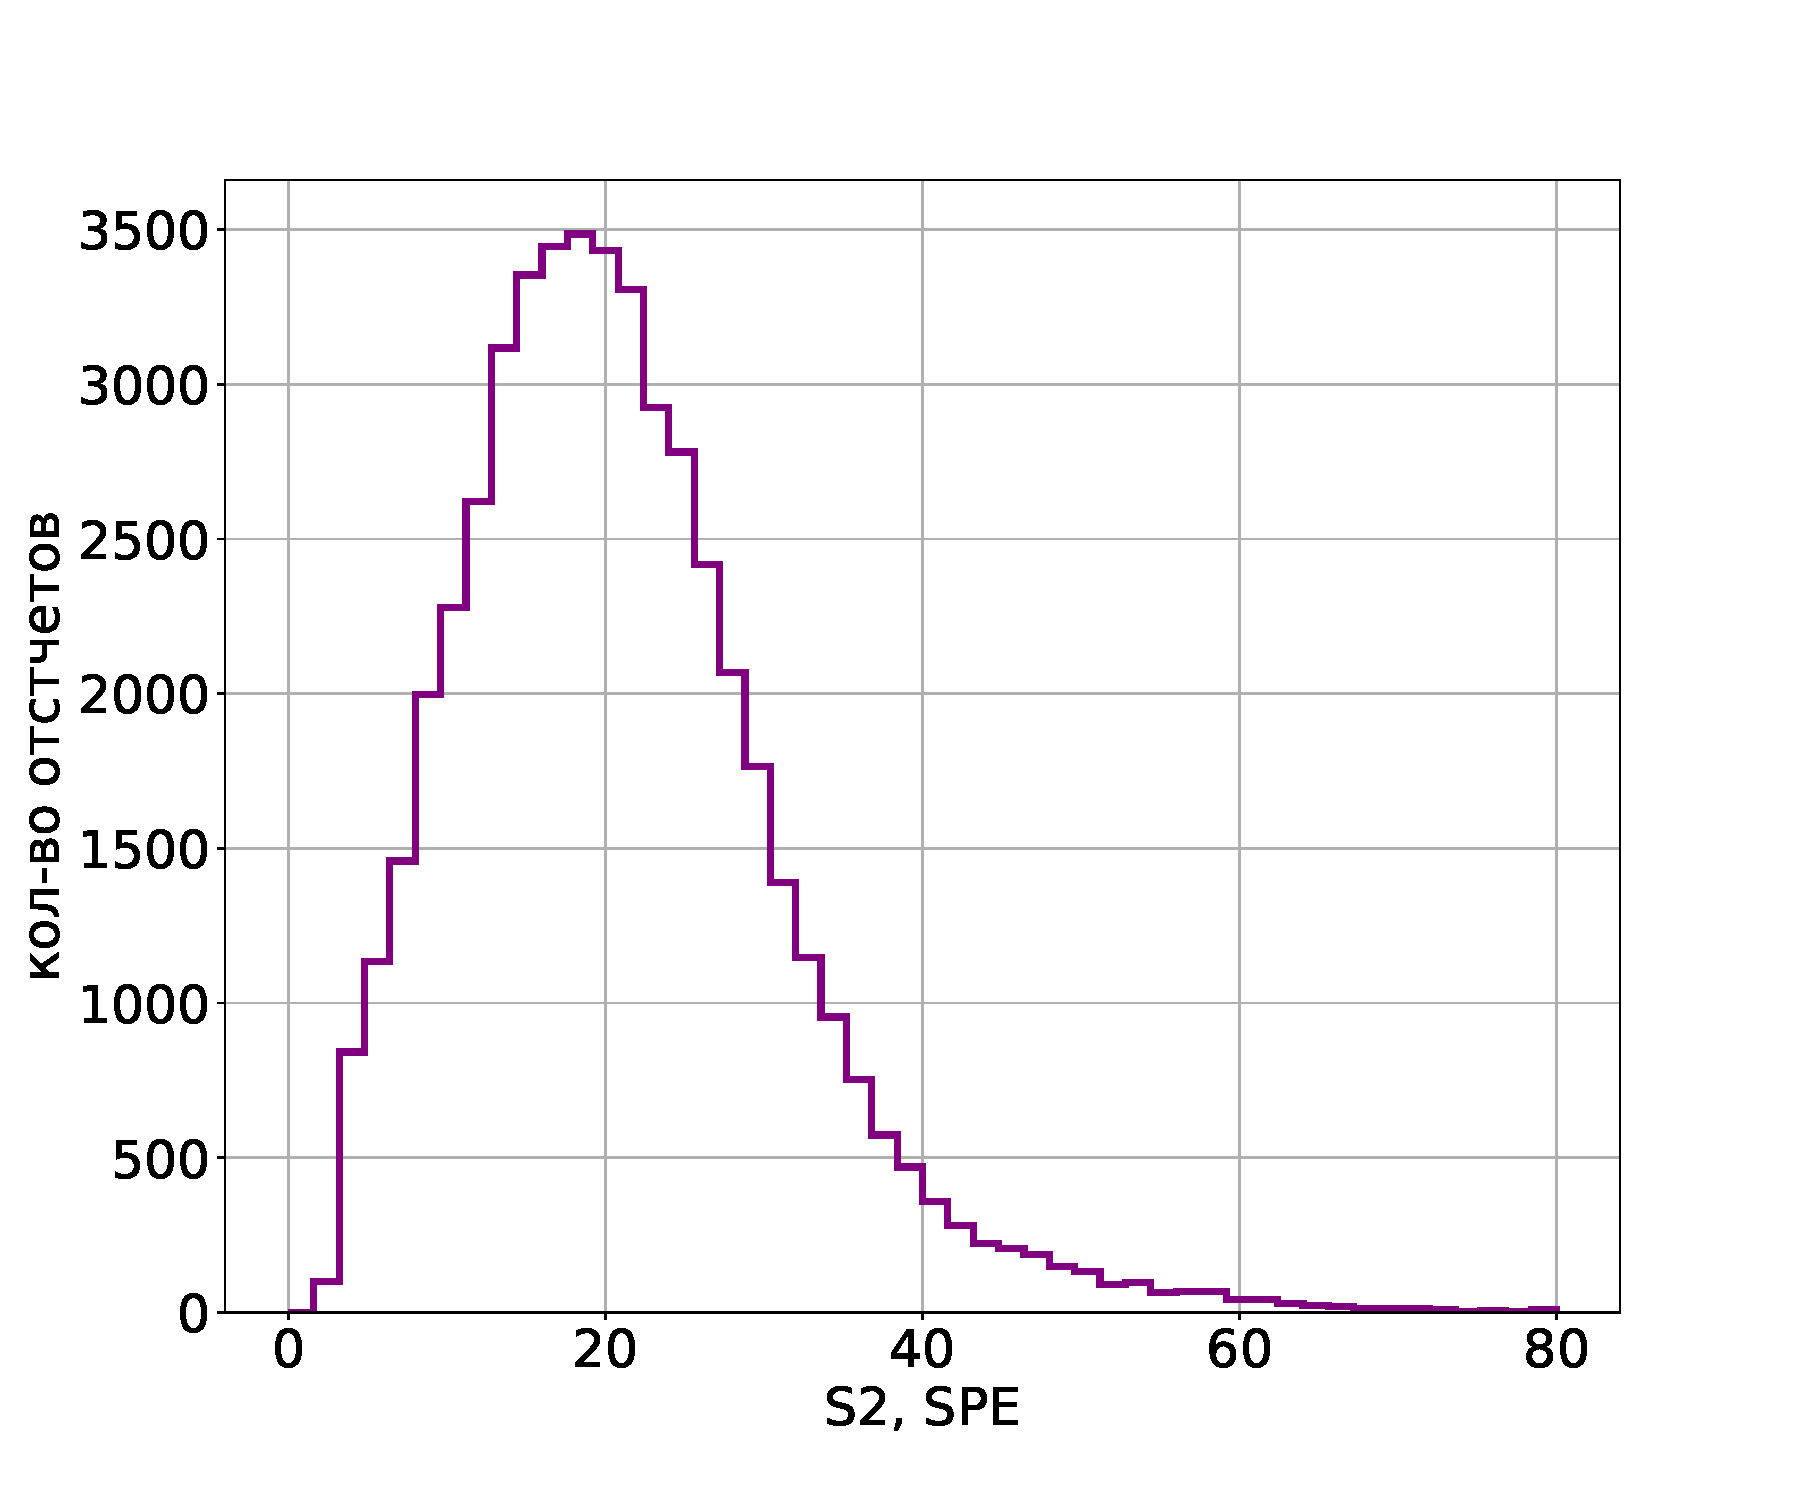
\includegraphics[width=1.0\linewidth]{images/se2022sp.pdf} \\ б)}
  \end{minipage}
  \caption{Распределения S2 в единицах SPE для SE-данных для инженерного сеанса (слева) и сеанса на КАЭС (справа)}
  \label{img:sespesp}  
\end{figure}

\textbf{Раздел 3.5} посвящен вычислению ионизационного выхода и коэффициента экстракции электронов с поверхности жидкого ксенона. 

Расчет ионизационного выхода (ionization yield -- IY) производился путем сравнения величины сигнала электролюминесценции от калибровочных гамма-источников и от одиночных электронов ионизации. Соответственно, для данной процедуры требуется выделение одиночного пика калибровочного гамма-источника. Так как разделение пиков $^{60}$Co возможно только в режиме антикорреляции, был использован пик меньшей энергии и данные SE сигналов. Значение ионизационного выхода рассчитывается по формуле:
\begin{equation}
    IY = k\cdot  \frac{A_{gamma\:source}}{A_{SE}\cdot E} \qquad \left[ \frac{e^-}{keV} \right],
    \label{formula:IY_calc_corr}
\end{equation}
где $A_{gamma\:source}$ и $A_{SE}$ -- положения пиков в фотоэлектронах после процедуры пространственного и энергетического восстановления, a $E$ -- энергия гамма-квантов соответствующего калибровочного источника, k -- поправочный коэффициент, связанный с вычислением площади малых импульсов.

В качестве калибровочного источника, пик от которого присутствует в расчетах, в ЛЭЯФ был использован $^{22}$Na c энергией гамма-квантов 511 кэВ, а при постановке эксперимента на КАЭС -- $^{137}$Cs с энергией гамма-квантов 662 кэВ. Так как расчет коэффициента экстракции электронов важен для предсказания спектра УКРН в детектор, на события был наложен дополнительный отбор на радиус от центра детектора (155 мм для инженерного сеанса и 130 мм для сеанса на КАЭС). Отбор событий, набранных во время сеанса на КАЭС совпадает с отбором, применявшимся для анализа УКРН-событий. Спектры S2 для гамма-калибровочных событий и для SE событий фитировались распределениями Гаусса для получения положений пиков.

Основная идея рассчета коэффициента экстракции электронов состоит в сравнении количества рожденных электронов в месте взаимодействия гамма-кванта с веществом и количества зарегистрированных электронов ионизации по S2. 
Значения величин ионизации для соответствующих энергий, были рассчитаны с использованием программного пакета NEST %версия?. 
\parПолученные значения ионизационного выхода и коэффициента экстракции электронов:
\begin{itemize}
    \item 2019: IY = 15.6$\pm$0.7 e/keV, EEE = 38$\pm$6.1\%
    \item 2022: IY = 12.9$\pm$0.7 e/keV, EEE = 34$\pm$5.9\%
\end{itemize}

Было произведено сравнение полученных значений с измерениями других коллабораций~\cite{Gouschin1978,AprileEEE_2014,Edwards_2018,PhysRevD.99.103024}. Результаты представлены на рисунке \ref{img:EEEworld}. Также на данном рисунке представлен расчет с использованием программного пакета NEST. Результаты, полученные в эксперименте РЭД-100 имеют тенденцию к отличию в большую сторону от общемировых значений. Вероятно, это связано с недостаточной точностью при расчете электрических полей в электролюминесцентном зазоре.

\begin{figure}[ht]
\center{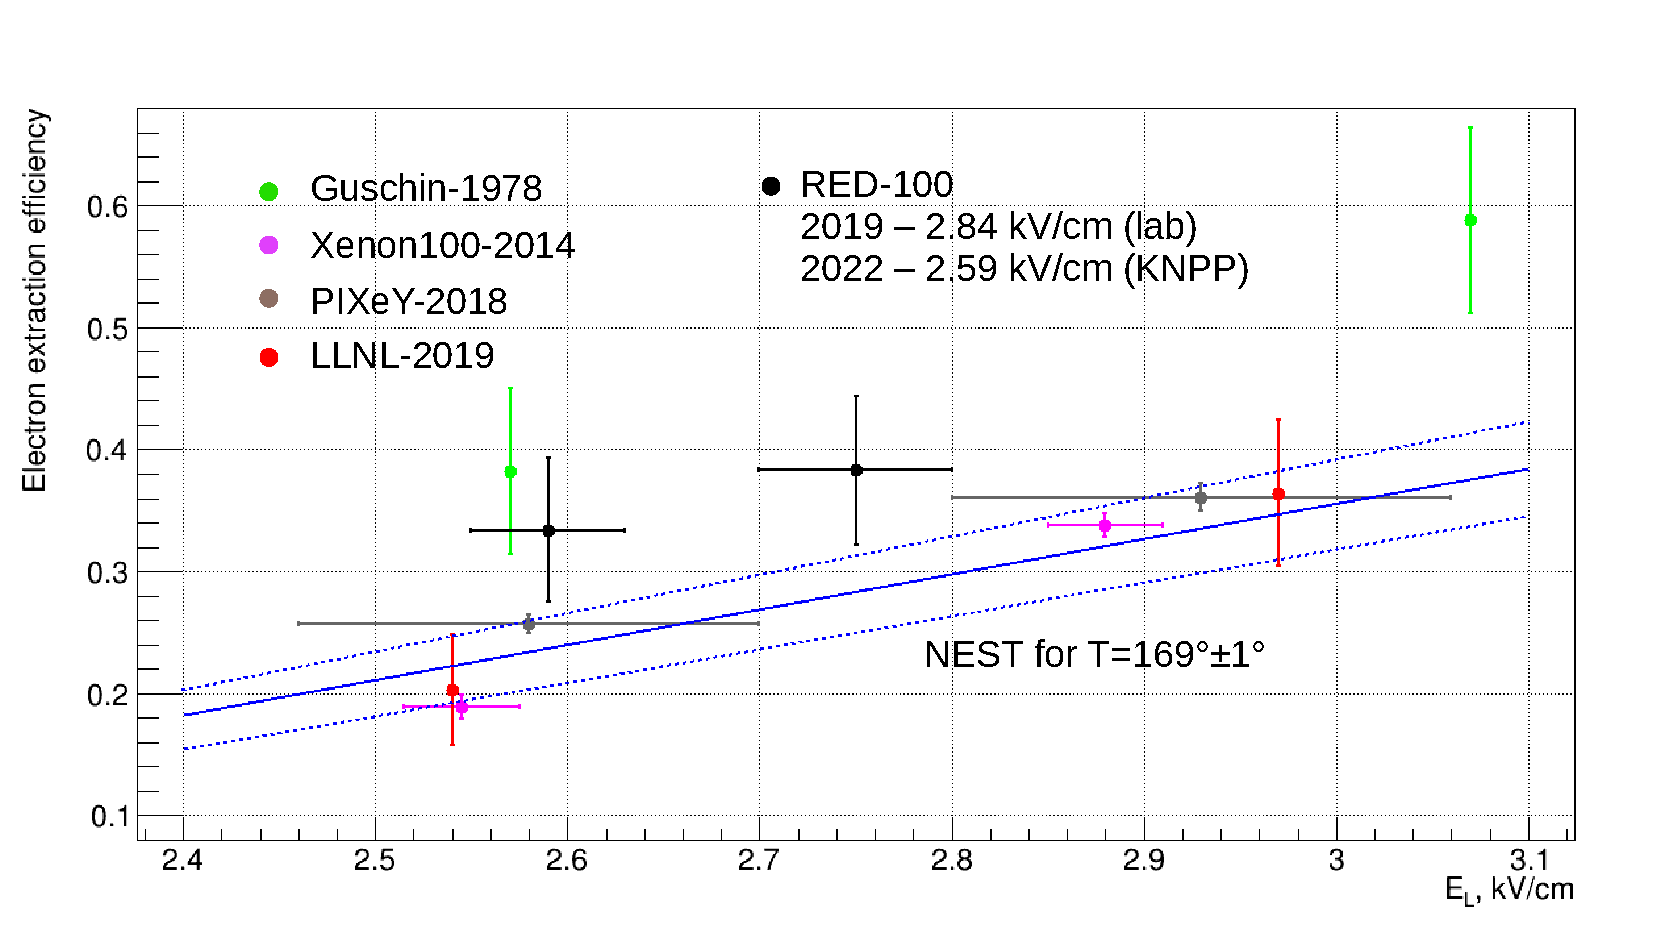
\includegraphics[width=1\linewidth]{images/RED_EEE_With_legend.pdf}}
  \caption{Сравнение результатов измерения ЕЕЕ в эксперименте РЭД-100 и другими коллаборациями, а также резульаты расчета данного коэффициента с использованием программного пакета NEST.}
  \label{img:EEEworld}  
\end{figure}

\underline{\textbf{Четвертая глава}} посвящена анализу физических данных эксперимента РЭД-100 на Калининской АЭС. 

В \textbf{разделе 4.1} описано моделирование ожидаемого сигнала от УКРН. Учитывая известную мощность реактора моделировался энергетический спектр ядер отдачи в GEANT-модели детектора, который далее пересчитывался в спектр, выраженный в электронах ионизации, который далее был скорректирован в соответствии с измеренными потерями при дрейфе и экстракции.

Далее, в соответствии процедурой моделирования временных разверток сигналов были смоделированы события в несколько электронов ионизации согласно полученному спектру. При моделировании использовались LRF, полученные при анализе измерений с гамма-источниками. Также была проведена процедура реконструкции координат и энергии данных событий. Для улучшения соотношения сигнал/шум при дальнейшем анализе к событиям были применены дополнительные отборы по длительности (<5 мкс) и радиусу (<130 мм), совпадающие с отборами для экспериментальных данных. Результирующий спектр восстановленной энергии смоделированных УКРН-событий представлен на рисунке \ref{img:cevnscpectrumspe}. 
\begin{figure}[ht]
\center{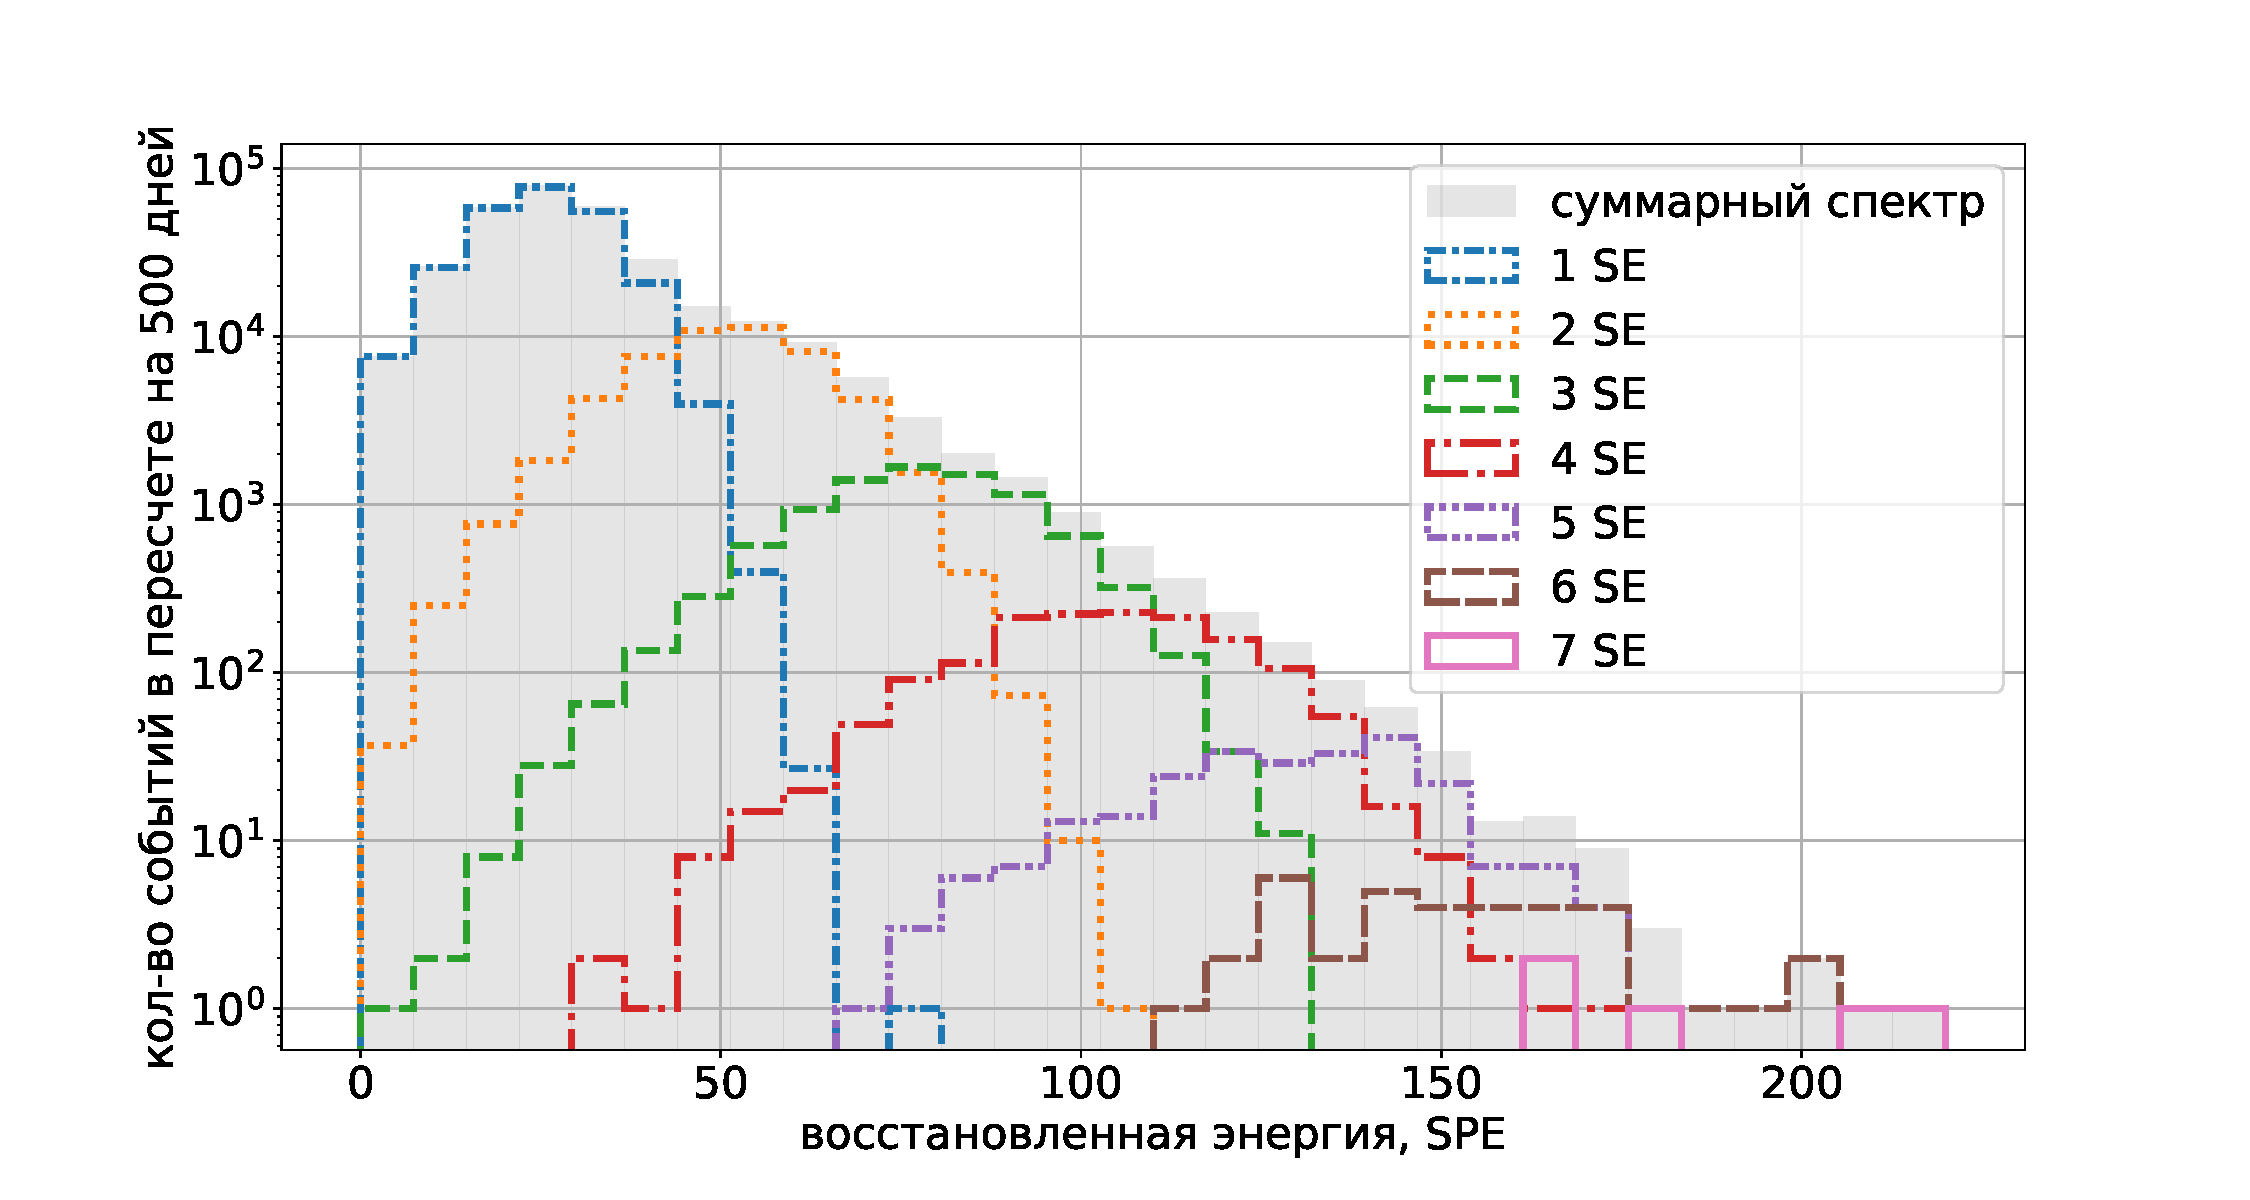
\includegraphics[width=1.0\linewidth]{images/cevnsspectrumSPE.pdf}}
	\caption{Спектр восстановленной энергии смоделирванных УКРН-событий.}
	\label{img:cevnscpectrumspe}
\end{figure}

\textbf{Разделе 4.2} посвящен кластеризации УКРН-подобных событий и отборам. Кластеризация событий в несколько электронов ионизации аналогична процедуре для SE-событий. Отличие заключалось в выборе пороговых значений для отбора импульсов, связанное с изменением SPE-калибровки. Кроме того, на события были наложены дополнительные отборы, описанные в данном разделе, учитывающие форму сигнала и отбор по радиусу (<130 мм). 

Существенную часть фона составляет совпадающие по времени сигналы от одного или нескольких спонтанно возникших электронов ионизации, как показано на рисунке~\ref{img:overlap}.
\begin{figure}[h]
\center{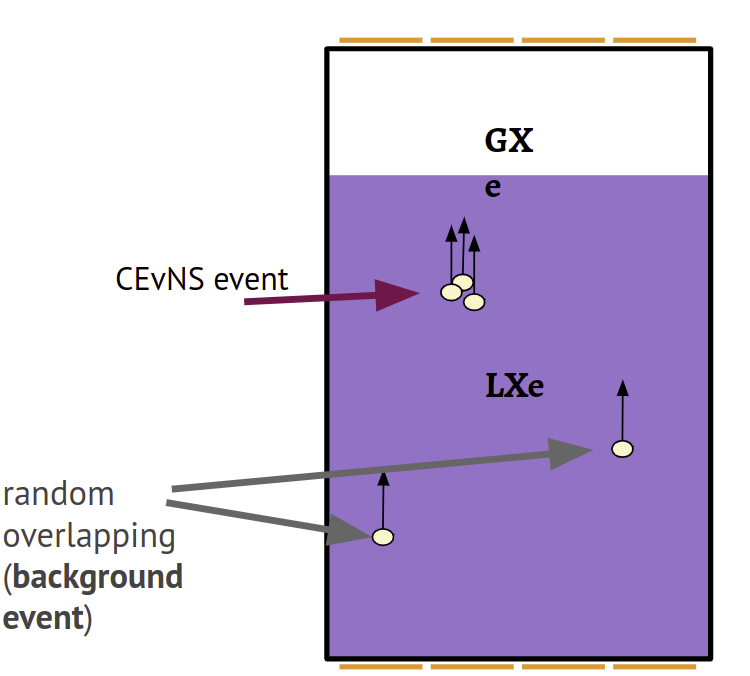
\includegraphics[width=0.5\linewidth]{images/randomoverlap.png}}
	\caption{Иллюстрация механизма возникновения событий совпадения.}
	\label{img:overlap}
\end{figure}

Для борьбы с такими событиями можно использовать идею о том, что точечные события не могут давать множественные вершины на плоскости XY. С целью подавления данной компоненты фона были применены технологии машинного обучения, а именно были разработаны две нейронные сети (перцептрон и сверточная нейронная сеть). Обучение сетей производилось на смоделированных событиях.

Результаты отбора УКРН событий и подавления фона, расчитанные по смоделированным данным приведены в таблицах~\ref{NNeffcevns}~и~\ref{NNeffbckg}. Для дальнейшего анализа отбирались события, идентифицированные обеими сетями как точечные.

\begin{table}[h]
    \centering
    \caption{Эффективности прохождения УКРН-событий для каждой из сетей, расчитанные по смоделированным данным.}  
\begin{tabular}{|c|c|c|c|c|}
\hline Количество SE & 3 & 4 & 5 & 6 \\
\hline сверточная сеть & $0.93$ & $0.96$ & $0.97$ & $0.98$ \\
\hline перцептрон & $0.88$ & $0.91$ & $0.93$ & $0.94$ \\
\hline
\end{tabular}
\label{NNeffcevns}
\end{table}

\begin{table}[h]
    \centering
    \caption{Эффективности подавления фоновых событий для каждой из сетей, расчитанные по смоделированным данным.}  
\begin{tabular}{|c|c|c|c|c|}
\hline Количество SE & 3 & 4 & 5 & 6 \\
\hline сверточная сеть & $0.87$ & $0.87$ & $0.93$ & $0.95$ \\
\hline перцептрон & $0.92$ & $0.93$ & $0.97$ & $0.98$ \\
\hline
\end{tabular}
\label{NNeffbckg}
\end{table}

Энергетический спектр фоновых событий до отборов по радиусу и точечности и после представлен на рисунке~\ref{img:bckgspecrtum}.
\begin{figure}[h]
\center{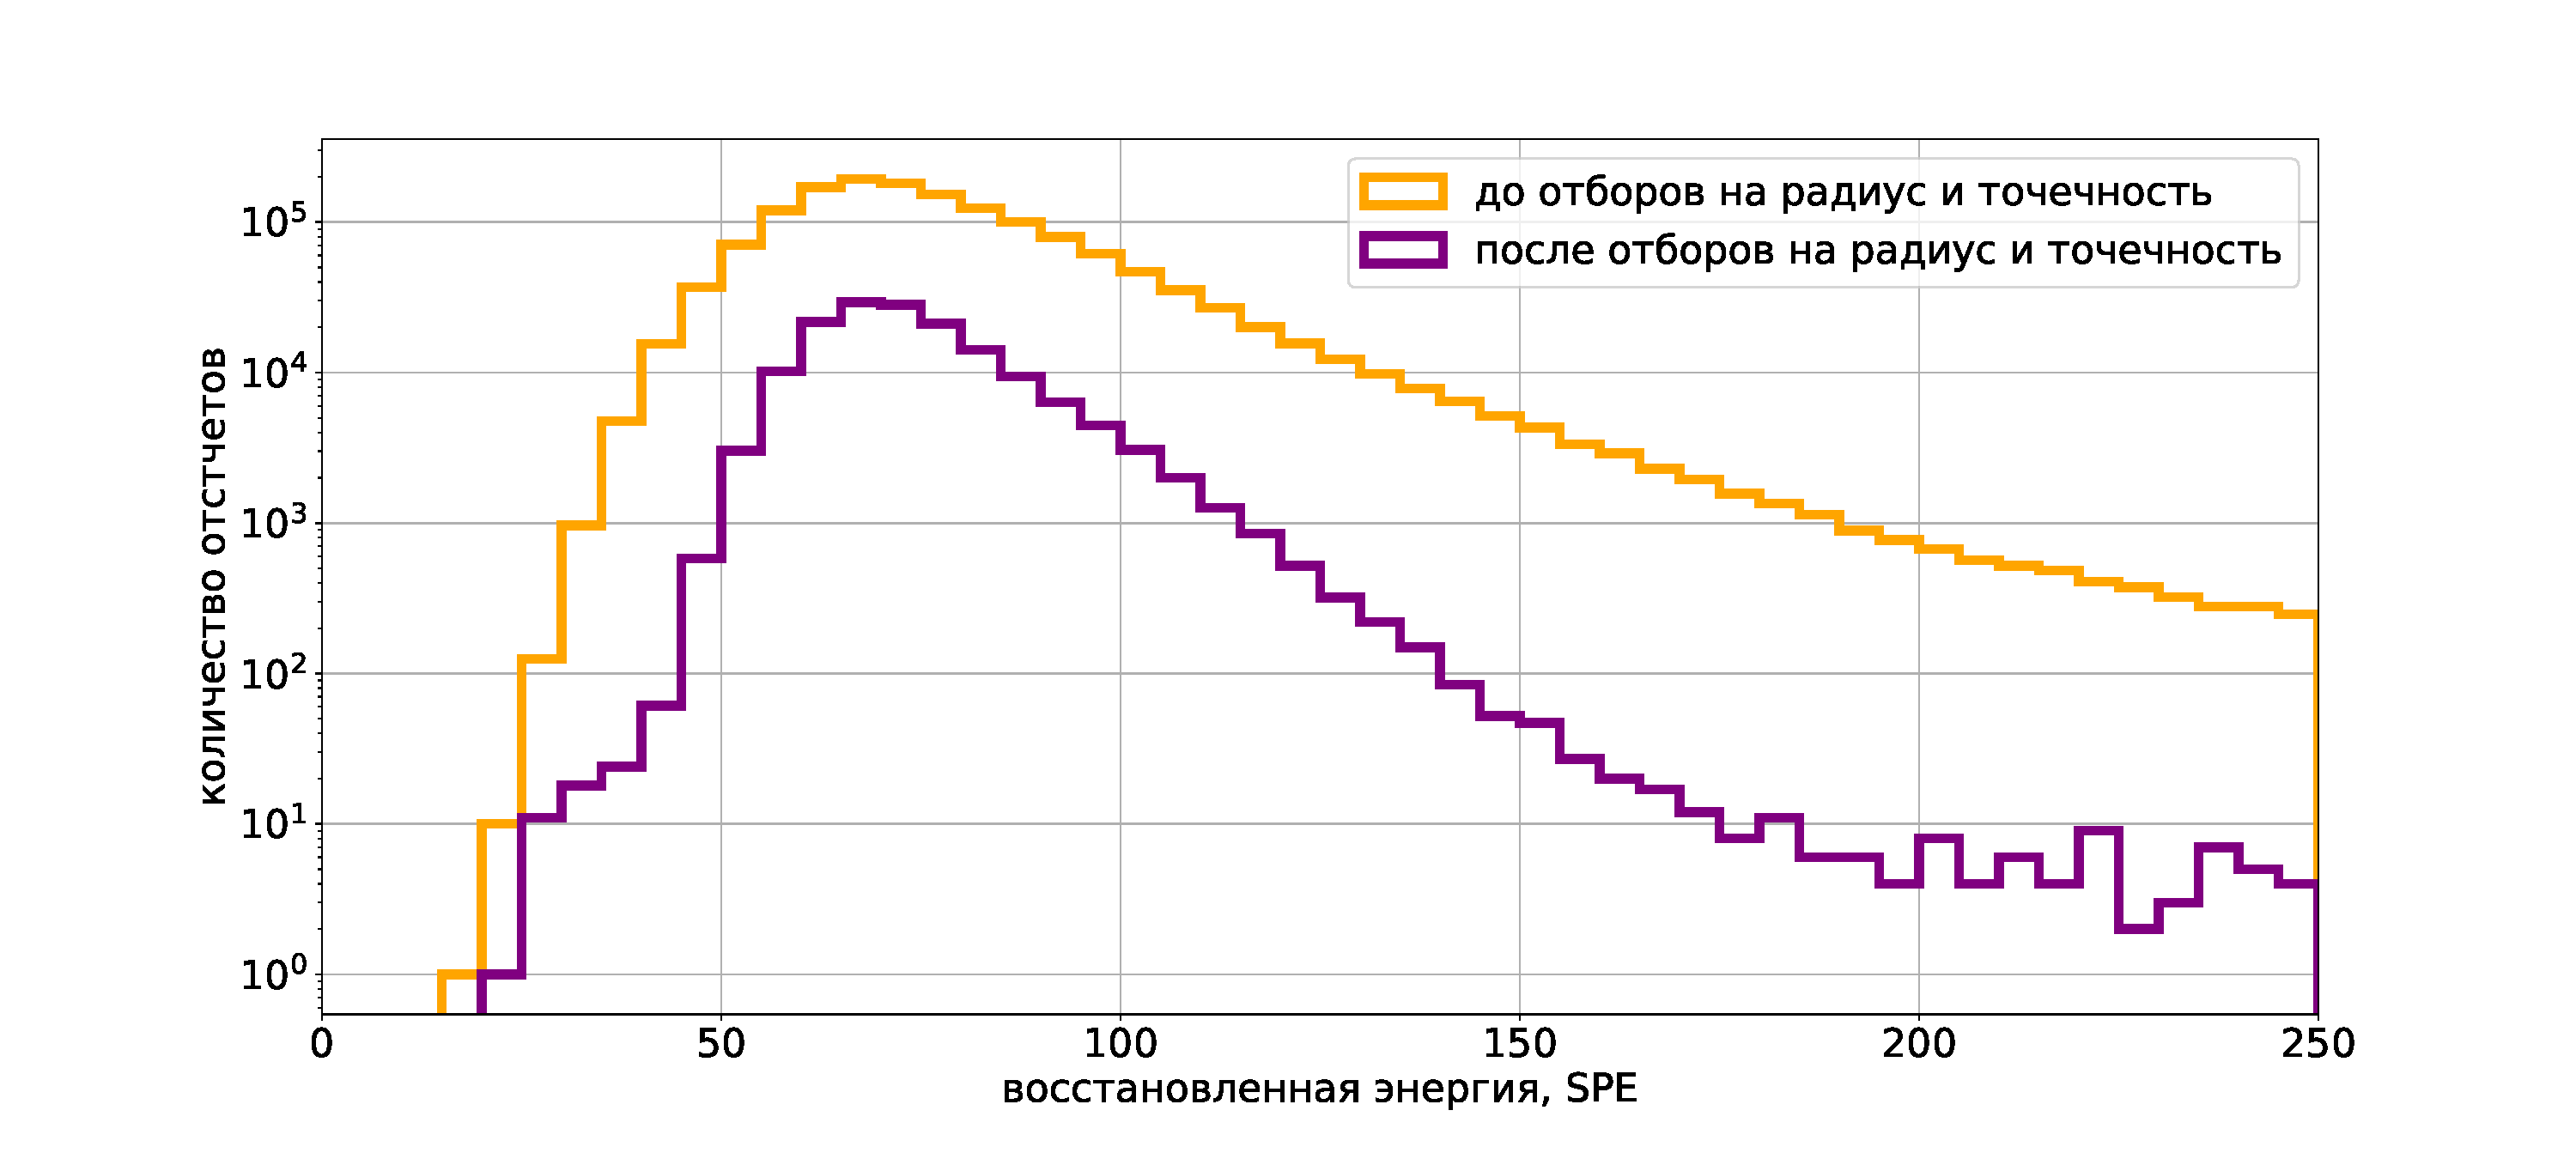
\includegraphics[width=0.8\linewidth]{images/cutsillustration.pdf}}
	\caption{Энергетический спектр фоновых событий до и после отборов по радиусу и точечности}
	\label{img:bckgspecrtum}
\end{figure}

\textbf{Разделе 4.2} посвящен анализу чувствительности детектора к предполагаемому сигналу УКРН. с учетом фонового сигнала. При этом для улучшения результата проводится анализ не только количества событий, но и формы спектра. Также учитывается живое время набора данных с выключенным ($\sim$22 часа) и включенным ($\sim$73 часа) реактором.
Процедура, примененная для анализа чувствительности в данной работе, описана в~\cite{Matt_thesis}. Для анализа был использован трехмерный спектр, где по трем осям были отложены восстановленная энергия, длительность и восстановленный радиус. Общая идея метода состоит в определении количества событий УКРН, которые с определенной пороговой вероятностью не могут быть имитированы случайными флуктуациями фона.

Полученное значение чувствительности ($\approx$37 событий УКРН в день) в $\approx$33 раз превышает предполагаемый уровень сигнала. Ожидаемое количество событий фона и сигнала приведено в таблице \ref{cevnscount}.

\begin{table}[hbt]
    \centering
    \caption{Ожидаемые скорости счета фона и сигнала (в день).}
    
\begin{tabular}{|c|c|c|c|c|}
\hline N e- & 3 & 4 & 5 & 6 \\
\hline bckg & $103 \mathrm{k}$ & $13.6 \mathrm{k}$ & 1268 & 150 \\
\hline CEvNS & $22.7$ & $4.7$ & $0.93$ & $0.19$ \\
\hline
\end{tabular}
\label{cevnscount}
\end{table}

В \underline{\textbf{заключении}} приведены основные результаты работы, которые заключаются в следующем:
%% Согласно ГОСТ Р 7.0.11-2011:
%% 5.3.3 В заключении диссертации излагают итоги выполненного исследования, рекомендации, перспективы дальнейшей разработки темы.
%% 9.2.3 В заключении автореферата диссертации излагают итоги данного исследования, рекомендации и перспективы дальнейшей разработки темы.
Основные результаты данной работы заключаются в следующем:
\begin{enumerate}
  \item Построена детальная оптическая модель детектора РЭД-100. На ее основе построена система моделирования временных разверток сигналов в несколько электронов ионизации в детекторе РЭД-100.
  \item На основе итеративного подхода получены функции распределения светосбора в детекторе РЭД-100 с использованием калибровочных данных с сеансов 2019 и 2022 годов. 
  \item Проведено пространственное восстановление событий в детекторе РЭД-100, на основе результатов было:
  \begin{itemize}
      \item Получено энергетическое разрешение детектора РЭД-100
      \item Получено значение ионизационного выхода
      \item Рассчитан коэффициент экстракции электронов с поверхности жидкого ксенона
  \end{itemize}
  \item Разработаны метод подавления фона неточечных событий на основе нейронных сетей с учетом временных разверток сигналов.
  \item Полученно предсказание сигнала от УКРН в детекторе РЭД-100
  \item Рассчитана чувствительность детектора РЭД-100 к сигналу УКРН
\end{enumerate}

\section*{Публикации автора по теме диссертации}
\begin{enumerate}
    \item First ground-level laboratory test of the two-phase xenon emission detector
RED-100 / D. Akimov [и др.] // Journal of Instrumentation. — 2020. —
февр. — т. 15, No 02. — P02020—P02020. — DOI: https://doi.org/10.1088/1748-0221/15/02/p02020
    \item The RED-100 experiment / D. Akimov [и др.] // Journal of
Instrumentation. — 2022. — нояб. — т. 17, No 11. — T11011. — DOI: 10.
1088/1748- 0221/17/11/T11011. — URL: https://dx.doi.org/10.
1088/1748-0221/17/11/T11011.
\end{enumerate}

%\newpage
%При использовании пакета \verb!biblatex! список публикаций автора по теме
%диссертации формируется в разделе <<\publications>>\ файла
%\verb!../common/characteristic.tex!  при помощи команды \verb!\nocite! 

\ifthenelse{\equal{\thebibliosel}{0}}{% Встроенная реализация с загрузкой файла через движок bibtex8
  \renewcommand{\refname}{\large \authorbibtitle}
  \nocite{*}
  \insertbiblioauthor                          % Подключаем Bib-базы
  \insertbiblioother   % !!! bibtex не умеет работать с несколькими библиографиями !!!
}{% Реализация пакетом biblatex через движок biber
  \insertbiblioauthor                          % Подключаем Bib-базы
  \insertbiblioother
}

